% **************************************************************************************************************
% A Classic Thesis Style
% An Homage to The Elements of Typographic Style
%
% Copyright (C) 2018 André Miede and Ivo Pletikosić
%
% If you like the style then I would appreciate a postcard. My address
% can be found in the file ClassicThesis.pdf. A collection of the
% postcards I received so far is available online at
% http://postcards.miede.de
%
% License:
% This program is free software; you can redistribute it and/or modify
% it under the terms of the GNU General Public License as published by
% the Free Software Foundation; either version 2 of the License, or
% (at your option) any later version.
%
% This program is distributed in the hope that it will be useful,
% but WITHOUT ANY WARRANTY; without even the implied warranty of
% MERCHANTABILITY or FITNESS FOR A PARTICULAR PURPOSE.  See the
% GNU General Public License for more details.
%
% You should have received a copy of the GNU General Public License
% along with this program; see the file COPYING.  If not, write to
% the Free Software Foundation, Inc., 59 Temple Place - Suite 330,
% Boston, MA 02111-1307, USA.
%
% PLEASE SEE ALSO THE AUTHORS' NOTE REGARDING THIS LICENSE
% IN THE DOCUMENTATION (ClassicThesis.pdf --> Chapter 1 / Chapter01.tex)
% **************************************************************************************************************
\RequirePackage{silence} % :-\
    \WarningFilter{scrreprt}{Usage of package `titlesec'}
    %\WarningFilter{scrreprt}{Activating an ugly workaround}
    \WarningFilter{titlesec}{Non standard sectioning command detected}
\documentclass[ twoside,openright,titlepage,numbers=noenddot,%1headlines,
                headinclude,footinclude,cleardoublepage=empty,abstract=on,
                BCOR=5mm,paper=a4,fontsize=11pt
                ]{scrreprt}

%********************************************************************
% Note: Make all your adjustments in here
%*******************************************************
% ****************************************************************************************************
% classicthesis-config.tex
% formerly known as loadpackages.sty, classicthesis-ldpkg.sty, and classicthesis-preamble.sty
% Use it at the beginning of your ClassicThesis.tex, or as a LaTeX Preamble
% in your ClassicThesis.{tex,lyx} with % ****************************************************************************************************
% classicthesis-config.tex
% formerly known as loadpackages.sty, classicthesis-ldpkg.sty, and classicthesis-preamble.sty
% Use it at the beginning of your ClassicThesis.tex, or as a LaTeX Preamble
% in your ClassicThesis.{tex,lyx} with % ****************************************************************************************************
% classicthesis-config.tex
% formerly known as loadpackages.sty, classicthesis-ldpkg.sty, and classicthesis-preamble.sty
% Use it at the beginning of your ClassicThesis.tex, or as a LaTeX Preamble
% in your ClassicThesis.{tex,lyx} with \input{classicthesis-config}
% ****************************************************************************************************
% If you like the classicthesis, then I would appreciate a postcard.
% My address can be found in the file ClassicThesis.pdf. A collection
% of the postcards I received so far is available online at
% http://postcards.miede.de
% ****************************************************************************************************


% ****************************************************************************************************
% 0. Set the encoding of your files. UTF-8 is the only sensible encoding nowadays. If you can't read
% äöüßáéçèê∂åëæƒÏ€ then change the encoding setting in your editor, not the line below. If your editor
% does not support utf8 use another editor!
% ****************************************************************************************************
\PassOptionsToPackage{utf8}{inputenc}
  \usepackage{inputenc}

\PassOptionsToPackage{T1}{fontenc} % T2A for cyrillics
  \usepackage{fontenc}


% ****************************************************************************************************
% 1. Configure classicthesis for your needs here, e.g., remove "drafting" below
% in order to deactivate the time-stamp on the pages
% (see ClassicThesis.pdf for more information):
% ****************************************************************************************************
\PassOptionsToPackage{
  drafting=true,    % print version information on the bottom of the pages
  tocaligned=false, % the left column of the toc will be aligned (no indentation)
  dottedtoc=false,  % page numbers in ToC flushed right
  eulerchapternumbers=true, % use AMS Euler for chapter font (otherwise Palatino)
  linedheaders=false,       % chaper headers will have line above and beneath
  floatperchapter=true,     % numbering per chapter for all floats (i.e., Figure 1.1)
  eulermath=false,  % use awesome Euler fonts for mathematical formulae (only with pdfLaTeX)
  beramono=true,    % toggle a nice monospaced font (w/ bold)
  palatino=true,    % deactivate standard font for loading another one, see the last section at the end of this file for suggestions
  style=classicthesis % classicthesis, arsclassica
}{classicthesis}


% ****************************************************************************************************
% 2. Personal data and user ad-hoc commands (insert your own data here)
% ****************************************************************************************************
\newcommand{\myTitle}{A Clean Title\xspace}
\newcommand{\mySubtitle}{A Fun Subtitle\xspace}
\newcommand{\myDegree}{Doktor-Ingenieur (Dr.-Ing.)\xspace}
\newcommand{\myName}{Lucas Kerbs\xspace}
\newcommand{\myProf}{Dr. Ryan Tully-Doyle\xspace}
\newcommand{\myOtherProf}{Put name here\xspace}
\newcommand{\mySupervisor}{Put name here\xspace}
\newcommand{\myFaculty}{Put data here\xspace}
\newcommand{\myDepartment}{Mathematics Department\xspace}
\newcommand{\myUni}{California Polytechnic University, San Luis Obispo\xspace}
\newcommand{\myLocation}{Saarbrücken\xspace}
\newcommand{\myTime}{February 2022\xspace}
\newcommand{\myVersion}{LucasThesis v1}

% ********************************************************************
% Setup, finetuning, and useful commands
% ********************************************************************
\providecommand{\mLyX}{L\kern-.1667em\lower.25em\hbox{Y}\kern-.125emX\@}
\newcommand{\ie}{i.\,e.}
\newcommand{\Ie}{I.\,e.}
\newcommand{\eg}{e.\,g.}
\newcommand{\Eg}{E.\,g.}
% ****************************************************************************************************


% ****************************************************************************************************
% 3. Loading some handy packages
% ****************************************************************************************************
% ********************************************************************
% Packages with options that might require adjustments
% ********************************************************************
\PassOptionsToPackage{ngerman,american}{babel} % change this to your language(s), main language last
% Spanish languages need extra options in order to work with this template
%\PassOptionsToPackage{spanish,es-lcroman}{babel}
    \usepackage{babel}

\usepackage{csquotes}
\PassOptionsToPackage{%
  %backend=biber,bibencoding=utf8, %instead of bibtex
  backend=bibtex8,bibencoding=ascii,%
  language=auto,%
  style=numeric-comp,%
  %style=authoryear-comp, % Author 1999, 2010
  %bibstyle=authoryear,dashed=false, % dashed: substitute rep. author with ---
  sorting=nyt, % name, year, title
  maxbibnames=10, % default: 3, et al.
  %backref=true,%
  natbib=true % natbib compatibility mode (\citep and \citet still work)
}{biblatex}
    \usepackage{biblatex}

\PassOptionsToPackage{fleqn}{amsmath}       % math environments and more by the AMS
  \usepackage{amsmath}

% ********************************************************************
% General useful packages
% ********************************************************************
\usepackage{graphicx} %
\usepackage{scrhack} % fix warnings when using KOMA with listings package
\usepackage{xspace} % to get the spacing after macros right
\PassOptionsToPackage{printonlyused,smaller}{acronym}
  \usepackage{acronym} % nice macros for handling all acronyms in the thesis
  %\renewcommand{\bflabel}[1]{{#1}\hfill} % fix the list of acronyms --> no longer working
  %\renewcommand*{\acsfont}[1]{\textsc{#1}}
  %\renewcommand*{\aclabelfont}[1]{\acsfont{#1}}
  %\def\bflabel#1{{#1\hfill}}
  \def\bflabel#1{{\acsfont{#1}\hfill}}
  \def\aclabelfont#1{\acsfont{#1}}
% ****************************************************************************************************
%\usepackage{pgfplots} % External TikZ/PGF support (thanks to Andreas Nautsch)
%\usetikzlibrary{external}
%\tikzexternalize[mode=list and make, prefix=ext-tikz/]
% ****************************************************************************************************


% ****************************************************************************************************
% 4. Setup floats: tables, (sub)figures, and captions
% ****************************************************************************************************
\usepackage{tabularx} % better tables
  \setlength{\extrarowheight}{3pt} % increase table row height
\newcommand{\tableheadline}[1]{\multicolumn{1}{l}{\spacedlowsmallcaps{#1}}}
\newcommand{\myfloatalign}{\centering} % to be used with each float for alignment
\usepackage{subfig}
% ****************************************************************************************************


% ****************************************************************************************************
% 5. Setup code listings
% ****************************************************************************************************
\usepackage{listings}
%\lstset{emph={trueIndex,root},emphstyle=\color{BlueViolet}}%\underbar} % for special keywords
\lstset{language=[LaTeX]Tex,%C++,
  morekeywords={PassOptionsToPackage,selectlanguage},
  keywordstyle=\color{RoyalBlue},%\bfseries,
  basicstyle=\small\ttfamily,
  %identifierstyle=\color{NavyBlue},
  commentstyle=\color{Green}\ttfamily,
  stringstyle=\rmfamily,
  numbers=none,%left,%
  numberstyle=\scriptsize,%\tiny
  stepnumber=5,
  numbersep=8pt,
  showstringspaces=false,
  breaklines=true,
  %frameround=ftff,
  %frame=single,
  belowcaptionskip=.75\baselineskip
  %frame=L
}
% ****************************************************************************************************




% ****************************************************************************************************
% 6. Last calls before the bar closes
% ****************************************************************************************************
% ********************************************************************
% Her Majesty herself
% ********************************************************************
\usepackage{classicthesis}


% ********************************************************************
% Fine-tune hyperreferences (hyperref should be called last)
% ********************************************************************
\hypersetup{%
  %draft, % hyperref's draft mode, for printing see below
  colorlinks=true, linktocpage=true, pdfstartpage=3, pdfstartview=FitV,%
  % uncomment the following line if you want to have black links (e.g., for printing)
  %colorlinks=false, linktocpage=false, pdfstartpage=3, pdfstartview=FitV, pdfborder={0 0 0},%
  breaklinks=true, pageanchor=true,%
  pdfpagemode=UseNone, %
  % pdfpagemode=UseOutlines,%
  plainpages=false, bookmarksnumbered, bookmarksopen=true, bookmarksopenlevel=1,%
  hypertexnames=true, pdfhighlight=/O,%nesting=true,%frenchlinks,%
  urlcolor=CTurl, linkcolor=CTlink, citecolor=CTcitation, %pagecolor=RoyalBlue,%
  %urlcolor=Black, linkcolor=Black, citecolor=Black, %pagecolor=Black,%
  pdftitle={\myTitle},%
  pdfauthor={\textcopyright\ \myName, \myUni, \myFaculty},%
  pdfsubject={},%
  pdfkeywords={},%
  pdfcreator={pdfLaTeX},%
  pdfproducer={LaTeX with hyperref and classicthesis}%
}


% ********************************************************************
% Setup autoreferences (hyperref and babel)
% ********************************************************************
% There are some issues regarding autorefnames
% http://www.tex.ac.uk/cgi-bin/texfaq2html?label=latexwords
% you have to redefine the macros for the
% language you use, e.g., american, ngerman
% (as chosen when loading babel/AtBeginDocument)
% ********************************************************************
\makeatletter
\@ifpackageloaded{babel}%
  {%
    \addto\extrasamerican{%
      \renewcommand*{\figureautorefname}{Figure}%
      \renewcommand*{\tableautorefname}{Table}%
      \renewcommand*{\partautorefname}{Part}%
      \renewcommand*{\chapterautorefname}{Chapter}%
      \renewcommand*{\sectionautorefname}{Section}%
      \renewcommand*{\subsectionautorefname}{Section}%
      \renewcommand*{\subsubsectionautorefname}{Section}%
    }%
    \addto\extrasngerman{%
      \renewcommand*{\paragraphautorefname}{Absatz}%
      \renewcommand*{\subparagraphautorefname}{Unterabsatz}%
      \renewcommand*{\footnoteautorefname}{Fu\"snote}%
      \renewcommand*{\FancyVerbLineautorefname}{Zeile}%
      \renewcommand*{\theoremautorefname}{Theorem}%
      \renewcommand*{\appendixautorefname}{Anhang}%
      \renewcommand*{\equationautorefname}{Gleichung}%
      \renewcommand*{\itemautorefname}{Punkt}%
    }%
      % Fix to getting autorefs for subfigures right (thanks to Belinda Vogt for changing the definition)
      \providecommand{\subfigureautorefname}{\figureautorefname}%
    }{\relax}
\makeatother


% ********************************************************************
% Development Stuff
% ********************************************************************
\listfiles
%\PassOptionsToPackage{l2tabu,orthodox,abort}{nag}
%  \usepackage{nag}
%\PassOptionsToPackage{warning, all}{onlyamsmath}
%  \usepackage{onlyamsmath}


% ****************************************************************************************************
% 7. Further adjustments (experimental)
% ****************************************************************************************************
% ********************************************************************
% Changing the text area
% ********************************************************************
%\areaset[current]{312pt}{761pt} % 686 (factor 2.2) + 33 head + 42 head \the\footskip
%\setlength{\marginparwidth}{7em}%
%\setlength{\marginparsep}{2em}%

% ********************************************************************
% Using different fonts
% ********************************************************************
%\usepackage[oldstylenums]{kpfonts} % oldstyle notextcomp
% \usepackage[osf]{libertine}
%\usepackage[light,condensed,math]{iwona}
%\renewcommand{\sfdefault}{iwona}
%\usepackage{lmodern} % <-- no osf support :-(
%\usepackage{cfr-lm} %
%\usepackage[urw-garamond]{mathdesign} <-- no osf support :-(
%\usepackage[default,osfigures]{opensans} % scale=0.95
%\usepackage[sfdefault]{FiraSans}
% \usepackage[opticals,mathlf]{MinionPro} % onlytext
% ********************************************************************
%\usepackage[largesc,osf]{newpxtext}
%\linespread{1.05} % a bit more for Palatino
% Used to fix these:
% https://bitbucket.org/amiede/classicthesis/issues/139/italics-in-pallatino-capitals-chapter
% https://bitbucket.org/amiede/classicthesis/issues/45/problema-testatine-su-classicthesis-style
% ********************************************************************
% ****************************************************************************************************

%% ADDED BY LUCAS 2/10 %%
\usepackage{amsmath,amsfonts,amssymb,amsthm, mathtools, mathrsfs, faktor, bbm}
\usepackage{wrapfig}
\usepackage{array}
\usepackage{graphicx}
\usepackage{tikz}
\usepackage{tikz-cd}
\usepackage{enumerate}

\usepackage{import}
\usepackage{xifthen}
\usepackage{pdfpages}
\usepackage{transparent}

\newtheorem{theorem}{Theorem}[part]
\newtheorem{corollary}{Corollary}[theorem]
\newtheorem{lemma}[theorem]{Lemma}
\newtheorem{definition}[theorem]{Definition}
\newtheorem{example}[theorem]{Example}

\newcommand{\incfig}[1]{%
  \def\svgwidth{0.5\columnwidth}
  \import{./images/}{#1.pdf_tex}
}
\newcommand*\circled[1]{\tikz[baseline=(char.base)]{
            \node[shape=circle,draw,inner sep=2pt] (char) {#1};}}
\definecolor{fgreen}{RGB}{34,169,75}
\definecolor{gpurple}{RGB}{152,68,158}


\newcommand{\im}{\mathrm{Im}}
\newcommand{\re}{\mathrm{Re}}
\newcommand{\res}{\mathrm{Res}}
\newcommand{\pv}{\mathrm{p.v.}}
\DeclareMathOperator{\tr}{tr}
\DeclareMathOperator{\Log}{Log}

\newcommand{\word}[1]{\quad \text{#1} \quad}
\newcommand{\dz}[1][z]{\hspace{2pt}\mathrm{d#1}}
\newcommand{\dx}[1][x]{\hspace{2pt}\mathrm{d#1}}
\newcommand{\paren}[1]{\left( #1 \right)}
\newcommand{\bracket}[1]{\left[ #1 \right]}
\newcommand{\cparen}[1]{\left\{ #1 \right\}}
\newcommand{\eval}[3]{\left. #1 \right|_{#2}^{#3}}
\newcommand{\abs}[1]{\left| #1 \right|}


% General shortcuts
\newcommand{\RR}{\mathbb{R}}
\newcommand{\CC}{\mathbb{C}}
\newcommand{\ZZ}{\mathbb{Z}}
\newcommand{\QQ}{\mathbb{Q}}
\newcommand{\NN}{\mathbb{N}}
\newcommand{\HH}{\mathbb{H}}
\newcommand{\MM}{\mathcal{M}}
\newcommand{\Id}{\mathbbm{1}}
\newcommand{\wms}{\textsc{wms} }
\newcommand{\wma}{\textsc{wma} }
\newcommand{\wwlog}{\textsc{wlog} }
\newcommand{\Arg}{\text{Arg}}
\renewcommand\qedsymbol{$\blacksquare$}

\usepackage{cleveref}

% ****************************************************************************************************
% If you like the classicthesis, then I would appreciate a postcard.
% My address can be found in the file ClassicThesis.pdf. A collection
% of the postcards I received so far is available online at
% http://postcards.miede.de
% ****************************************************************************************************


% ****************************************************************************************************
% 0. Set the encoding of your files. UTF-8 is the only sensible encoding nowadays. If you can't read
% äöüßáéçèê∂åëæƒÏ€ then change the encoding setting in your editor, not the line below. If your editor
% does not support utf8 use another editor!
% ****************************************************************************************************
\PassOptionsToPackage{utf8}{inputenc}
  \usepackage{inputenc}

\PassOptionsToPackage{T1}{fontenc} % T2A for cyrillics
  \usepackage{fontenc}


% ****************************************************************************************************
% 1. Configure classicthesis for your needs here, e.g., remove "drafting" below
% in order to deactivate the time-stamp on the pages
% (see ClassicThesis.pdf for more information):
% ****************************************************************************************************
\PassOptionsToPackage{
  drafting=true,    % print version information on the bottom of the pages
  tocaligned=false, % the left column of the toc will be aligned (no indentation)
  dottedtoc=false,  % page numbers in ToC flushed right
  eulerchapternumbers=true, % use AMS Euler for chapter font (otherwise Palatino)
  linedheaders=false,       % chaper headers will have line above and beneath
  floatperchapter=true,     % numbering per chapter for all floats (i.e., Figure 1.1)
  eulermath=false,  % use awesome Euler fonts for mathematical formulae (only with pdfLaTeX)
  beramono=true,    % toggle a nice monospaced font (w/ bold)
  palatino=true,    % deactivate standard font for loading another one, see the last section at the end of this file for suggestions
  style=classicthesis % classicthesis, arsclassica
}{classicthesis}


% ****************************************************************************************************
% 2. Personal data and user ad-hoc commands (insert your own data here)
% ****************************************************************************************************
\newcommand{\myTitle}{A Clean Title\xspace}
\newcommand{\mySubtitle}{A Fun Subtitle\xspace}
\newcommand{\myDegree}{Doktor-Ingenieur (Dr.-Ing.)\xspace}
\newcommand{\myName}{Lucas Kerbs\xspace}
\newcommand{\myProf}{Dr. Ryan Tully-Doyle\xspace}
\newcommand{\myOtherProf}{Put name here\xspace}
\newcommand{\mySupervisor}{Put name here\xspace}
\newcommand{\myFaculty}{Put data here\xspace}
\newcommand{\myDepartment}{Mathematics Department\xspace}
\newcommand{\myUni}{California Polytechnic University, San Luis Obispo\xspace}
\newcommand{\myLocation}{Saarbrücken\xspace}
\newcommand{\myTime}{February 2022\xspace}
\newcommand{\myVersion}{LucasThesis v1}

% ********************************************************************
% Setup, finetuning, and useful commands
% ********************************************************************
\providecommand{\mLyX}{L\kern-.1667em\lower.25em\hbox{Y}\kern-.125emX\@}
\newcommand{\ie}{i.\,e.}
\newcommand{\Ie}{I.\,e.}
\newcommand{\eg}{e.\,g.}
\newcommand{\Eg}{E.\,g.}
% ****************************************************************************************************


% ****************************************************************************************************
% 3. Loading some handy packages
% ****************************************************************************************************
% ********************************************************************
% Packages with options that might require adjustments
% ********************************************************************
\PassOptionsToPackage{ngerman,american}{babel} % change this to your language(s), main language last
% Spanish languages need extra options in order to work with this template
%\PassOptionsToPackage{spanish,es-lcroman}{babel}
    \usepackage{babel}

\usepackage{csquotes}
\PassOptionsToPackage{%
  %backend=biber,bibencoding=utf8, %instead of bibtex
  backend=bibtex8,bibencoding=ascii,%
  language=auto,%
  style=numeric-comp,%
  %style=authoryear-comp, % Author 1999, 2010
  %bibstyle=authoryear,dashed=false, % dashed: substitute rep. author with ---
  sorting=nyt, % name, year, title
  maxbibnames=10, % default: 3, et al.
  %backref=true,%
  natbib=true % natbib compatibility mode (\citep and \citet still work)
}{biblatex}
    \usepackage{biblatex}

\PassOptionsToPackage{fleqn}{amsmath}       % math environments and more by the AMS
  \usepackage{amsmath}

% ********************************************************************
% General useful packages
% ********************************************************************
\usepackage{graphicx} %
\usepackage{scrhack} % fix warnings when using KOMA with listings package
\usepackage{xspace} % to get the spacing after macros right
\PassOptionsToPackage{printonlyused,smaller}{acronym}
  \usepackage{acronym} % nice macros for handling all acronyms in the thesis
  %\renewcommand{\bflabel}[1]{{#1}\hfill} % fix the list of acronyms --> no longer working
  %\renewcommand*{\acsfont}[1]{\textsc{#1}}
  %\renewcommand*{\aclabelfont}[1]{\acsfont{#1}}
  %\def\bflabel#1{{#1\hfill}}
  \def\bflabel#1{{\acsfont{#1}\hfill}}
  \def\aclabelfont#1{\acsfont{#1}}
% ****************************************************************************************************
%\usepackage{pgfplots} % External TikZ/PGF support (thanks to Andreas Nautsch)
%\usetikzlibrary{external}
%\tikzexternalize[mode=list and make, prefix=ext-tikz/]
% ****************************************************************************************************


% ****************************************************************************************************
% 4. Setup floats: tables, (sub)figures, and captions
% ****************************************************************************************************
\usepackage{tabularx} % better tables
  \setlength{\extrarowheight}{3pt} % increase table row height
\newcommand{\tableheadline}[1]{\multicolumn{1}{l}{\spacedlowsmallcaps{#1}}}
\newcommand{\myfloatalign}{\centering} % to be used with each float for alignment
\usepackage{subfig}
% ****************************************************************************************************


% ****************************************************************************************************
% 5. Setup code listings
% ****************************************************************************************************
\usepackage{listings}
%\lstset{emph={trueIndex,root},emphstyle=\color{BlueViolet}}%\underbar} % for special keywords
\lstset{language=[LaTeX]Tex,%C++,
  morekeywords={PassOptionsToPackage,selectlanguage},
  keywordstyle=\color{RoyalBlue},%\bfseries,
  basicstyle=\small\ttfamily,
  %identifierstyle=\color{NavyBlue},
  commentstyle=\color{Green}\ttfamily,
  stringstyle=\rmfamily,
  numbers=none,%left,%
  numberstyle=\scriptsize,%\tiny
  stepnumber=5,
  numbersep=8pt,
  showstringspaces=false,
  breaklines=true,
  %frameround=ftff,
  %frame=single,
  belowcaptionskip=.75\baselineskip
  %frame=L
}
% ****************************************************************************************************




% ****************************************************************************************************
% 6. Last calls before the bar closes
% ****************************************************************************************************
% ********************************************************************
% Her Majesty herself
% ********************************************************************
\usepackage{classicthesis}


% ********************************************************************
% Fine-tune hyperreferences (hyperref should be called last)
% ********************************************************************
\hypersetup{%
  %draft, % hyperref's draft mode, for printing see below
  colorlinks=true, linktocpage=true, pdfstartpage=3, pdfstartview=FitV,%
  % uncomment the following line if you want to have black links (e.g., for printing)
  %colorlinks=false, linktocpage=false, pdfstartpage=3, pdfstartview=FitV, pdfborder={0 0 0},%
  breaklinks=true, pageanchor=true,%
  pdfpagemode=UseNone, %
  % pdfpagemode=UseOutlines,%
  plainpages=false, bookmarksnumbered, bookmarksopen=true, bookmarksopenlevel=1,%
  hypertexnames=true, pdfhighlight=/O,%nesting=true,%frenchlinks,%
  urlcolor=CTurl, linkcolor=CTlink, citecolor=CTcitation, %pagecolor=RoyalBlue,%
  %urlcolor=Black, linkcolor=Black, citecolor=Black, %pagecolor=Black,%
  pdftitle={\myTitle},%
  pdfauthor={\textcopyright\ \myName, \myUni, \myFaculty},%
  pdfsubject={},%
  pdfkeywords={},%
  pdfcreator={pdfLaTeX},%
  pdfproducer={LaTeX with hyperref and classicthesis}%
}


% ********************************************************************
% Setup autoreferences (hyperref and babel)
% ********************************************************************
% There are some issues regarding autorefnames
% http://www.tex.ac.uk/cgi-bin/texfaq2html?label=latexwords
% you have to redefine the macros for the
% language you use, e.g., american, ngerman
% (as chosen when loading babel/AtBeginDocument)
% ********************************************************************
\makeatletter
\@ifpackageloaded{babel}%
  {%
    \addto\extrasamerican{%
      \renewcommand*{\figureautorefname}{Figure}%
      \renewcommand*{\tableautorefname}{Table}%
      \renewcommand*{\partautorefname}{Part}%
      \renewcommand*{\chapterautorefname}{Chapter}%
      \renewcommand*{\sectionautorefname}{Section}%
      \renewcommand*{\subsectionautorefname}{Section}%
      \renewcommand*{\subsubsectionautorefname}{Section}%
    }%
    \addto\extrasngerman{%
      \renewcommand*{\paragraphautorefname}{Absatz}%
      \renewcommand*{\subparagraphautorefname}{Unterabsatz}%
      \renewcommand*{\footnoteautorefname}{Fu\"snote}%
      \renewcommand*{\FancyVerbLineautorefname}{Zeile}%
      \renewcommand*{\theoremautorefname}{Theorem}%
      \renewcommand*{\appendixautorefname}{Anhang}%
      \renewcommand*{\equationautorefname}{Gleichung}%
      \renewcommand*{\itemautorefname}{Punkt}%
    }%
      % Fix to getting autorefs for subfigures right (thanks to Belinda Vogt for changing the definition)
      \providecommand{\subfigureautorefname}{\figureautorefname}%
    }{\relax}
\makeatother


% ********************************************************************
% Development Stuff
% ********************************************************************
\listfiles
%\PassOptionsToPackage{l2tabu,orthodox,abort}{nag}
%  \usepackage{nag}
%\PassOptionsToPackage{warning, all}{onlyamsmath}
%  \usepackage{onlyamsmath}


% ****************************************************************************************************
% 7. Further adjustments (experimental)
% ****************************************************************************************************
% ********************************************************************
% Changing the text area
% ********************************************************************
%\areaset[current]{312pt}{761pt} % 686 (factor 2.2) + 33 head + 42 head \the\footskip
%\setlength{\marginparwidth}{7em}%
%\setlength{\marginparsep}{2em}%

% ********************************************************************
% Using different fonts
% ********************************************************************
%\usepackage[oldstylenums]{kpfonts} % oldstyle notextcomp
% \usepackage[osf]{libertine}
%\usepackage[light,condensed,math]{iwona}
%\renewcommand{\sfdefault}{iwona}
%\usepackage{lmodern} % <-- no osf support :-(
%\usepackage{cfr-lm} %
%\usepackage[urw-garamond]{mathdesign} <-- no osf support :-(
%\usepackage[default,osfigures]{opensans} % scale=0.95
%\usepackage[sfdefault]{FiraSans}
% \usepackage[opticals,mathlf]{MinionPro} % onlytext
% ********************************************************************
%\usepackage[largesc,osf]{newpxtext}
%\linespread{1.05} % a bit more for Palatino
% Used to fix these:
% https://bitbucket.org/amiede/classicthesis/issues/139/italics-in-pallatino-capitals-chapter
% https://bitbucket.org/amiede/classicthesis/issues/45/problema-testatine-su-classicthesis-style
% ********************************************************************
% ****************************************************************************************************

%% ADDED BY LUCAS 2/10 %%
\usepackage{amsmath,amsfonts,amssymb,amsthm, mathtools, mathrsfs, faktor, bbm}
\usepackage{wrapfig}
\usepackage{array}
\usepackage{graphicx}
\usepackage{tikz}
\usepackage{tikz-cd}
\usepackage{enumerate}

\usepackage{import}
\usepackage{xifthen}
\usepackage{pdfpages}
\usepackage{transparent}

\newtheorem{theorem}{Theorem}[part]
\newtheorem{corollary}{Corollary}[theorem]
\newtheorem{lemma}[theorem]{Lemma}
\newtheorem{definition}[theorem]{Definition}
\newtheorem{example}[theorem]{Example}

\newcommand{\incfig}[1]{%
  \def\svgwidth{0.5\columnwidth}
  \import{./images/}{#1.pdf_tex}
}
\newcommand*\circled[1]{\tikz[baseline=(char.base)]{
            \node[shape=circle,draw,inner sep=2pt] (char) {#1};}}
\definecolor{fgreen}{RGB}{34,169,75}
\definecolor{gpurple}{RGB}{152,68,158}


\newcommand{\im}{\mathrm{Im}}
\newcommand{\re}{\mathrm{Re}}
\newcommand{\res}{\mathrm{Res}}
\newcommand{\pv}{\mathrm{p.v.}}
\DeclareMathOperator{\tr}{tr}
\DeclareMathOperator{\Log}{Log}

\newcommand{\word}[1]{\quad \text{#1} \quad}
\newcommand{\dz}[1][z]{\hspace{2pt}\mathrm{d#1}}
\newcommand{\dx}[1][x]{\hspace{2pt}\mathrm{d#1}}
\newcommand{\paren}[1]{\left( #1 \right)}
\newcommand{\bracket}[1]{\left[ #1 \right]}
\newcommand{\cparen}[1]{\left\{ #1 \right\}}
\newcommand{\eval}[3]{\left. #1 \right|_{#2}^{#3}}
\newcommand{\abs}[1]{\left| #1 \right|}


% General shortcuts
\newcommand{\RR}{\mathbb{R}}
\newcommand{\CC}{\mathbb{C}}
\newcommand{\ZZ}{\mathbb{Z}}
\newcommand{\QQ}{\mathbb{Q}}
\newcommand{\NN}{\mathbb{N}}
\newcommand{\HH}{\mathbb{H}}
\newcommand{\MM}{\mathcal{M}}
\newcommand{\Id}{\mathbbm{1}}
\newcommand{\wms}{\textsc{wms} }
\newcommand{\wma}{\textsc{wma} }
\newcommand{\wwlog}{\textsc{wlog} }
\newcommand{\Arg}{\text{Arg}}
\renewcommand\qedsymbol{$\blacksquare$}

\usepackage{cleveref}

% ****************************************************************************************************
% If you like the classicthesis, then I would appreciate a postcard.
% My address can be found in the file ClassicThesis.pdf. A collection
% of the postcards I received so far is available online at
% http://postcards.miede.de
% ****************************************************************************************************


% ****************************************************************************************************
% 0. Set the encoding of your files. UTF-8 is the only sensible encoding nowadays. If you can't read
% äöüßáéçèê∂åëæƒÏ€ then change the encoding setting in your editor, not the line below. If your editor
% does not support utf8 use another editor!
% ****************************************************************************************************
\PassOptionsToPackage{utf8}{inputenc}
  \usepackage{inputenc}

\PassOptionsToPackage{T1}{fontenc} % T2A for cyrillics
  \usepackage{fontenc}


% ****************************************************************************************************
% 1. Configure classicthesis for your needs here, e.g., remove "drafting" below
% in order to deactivate the time-stamp on the pages
% (see ClassicThesis.pdf for more information):
% ****************************************************************************************************
\PassOptionsToPackage{
  drafting=true,    % print version information on the bottom of the pages
  tocaligned=false, % the left column of the toc will be aligned (no indentation)
  dottedtoc=false,  % page numbers in ToC flushed right
  eulerchapternumbers=true, % use AMS Euler for chapter font (otherwise Palatino)
  linedheaders=false,       % chaper headers will have line above and beneath
  floatperchapter=true,     % numbering per chapter for all floats (i.e., Figure 1.1)
  eulermath=false,  % use awesome Euler fonts for mathematical formulae (only with pdfLaTeX)
  beramono=true,    % toggle a nice monospaced font (w/ bold)
  palatino=true,    % deactivate standard font for loading another one, see the last section at the end of this file for suggestions
  style=classicthesis % classicthesis, arsclassica
}{classicthesis}


% ****************************************************************************************************
% 2. Personal data and user ad-hoc commands (insert your own data here)
% ****************************************************************************************************
\newcommand{\myTitle}{A Clean Title\xspace}
\newcommand{\mySubtitle}{A Fun Subtitle\xspace}
\newcommand{\myDegree}{Doktor-Ingenieur (Dr.-Ing.)\xspace}
\newcommand{\myName}{Lucas Kerbs\xspace}
\newcommand{\myProf}{Dr. Ryan Tully-Doyle\xspace}
\newcommand{\myOtherProf}{Put name here\xspace}
\newcommand{\mySupervisor}{Put name here\xspace}
\newcommand{\myFaculty}{Put data here\xspace}
\newcommand{\myDepartment}{Mathematics Department\xspace}
\newcommand{\myUni}{California Polytechnic University, San Luis Obispo\xspace}
\newcommand{\myLocation}{Saarbrücken\xspace}
\newcommand{\myTime}{February 2022\xspace}
\newcommand{\myVersion}{LucasThesis v1}

% ********************************************************************
% Setup, finetuning, and useful commands
% ********************************************************************
\providecommand{\mLyX}{L\kern-.1667em\lower.25em\hbox{Y}\kern-.125emX\@}
\newcommand{\ie}{i.\,e.}
\newcommand{\Ie}{I.\,e.}
\newcommand{\eg}{e.\,g.}
\newcommand{\Eg}{E.\,g.}
% ****************************************************************************************************


% ****************************************************************************************************
% 3. Loading some handy packages
% ****************************************************************************************************
% ********************************************************************
% Packages with options that might require adjustments
% ********************************************************************
\PassOptionsToPackage{ngerman,american}{babel} % change this to your language(s), main language last
% Spanish languages need extra options in order to work with this template
%\PassOptionsToPackage{spanish,es-lcroman}{babel}
    \usepackage{babel}

\usepackage{csquotes}
\PassOptionsToPackage{%
  %backend=biber,bibencoding=utf8, %instead of bibtex
  backend=bibtex8,bibencoding=ascii,%
  language=auto,%
  style=numeric-comp,%
  %style=authoryear-comp, % Author 1999, 2010
  %bibstyle=authoryear,dashed=false, % dashed: substitute rep. author with ---
  sorting=nyt, % name, year, title
  maxbibnames=10, % default: 3, et al.
  %backref=true,%
  natbib=true % natbib compatibility mode (\citep and \citet still work)
}{biblatex}
    \usepackage{biblatex}

\PassOptionsToPackage{fleqn}{amsmath}       % math environments and more by the AMS
  \usepackage{amsmath}

% ********************************************************************
% General useful packages
% ********************************************************************
\usepackage{graphicx} %
\usepackage{scrhack} % fix warnings when using KOMA with listings package
\usepackage{xspace} % to get the spacing after macros right
\PassOptionsToPackage{printonlyused,smaller}{acronym}
  \usepackage{acronym} % nice macros for handling all acronyms in the thesis
  %\renewcommand{\bflabel}[1]{{#1}\hfill} % fix the list of acronyms --> no longer working
  %\renewcommand*{\acsfont}[1]{\textsc{#1}}
  %\renewcommand*{\aclabelfont}[1]{\acsfont{#1}}
  %\def\bflabel#1{{#1\hfill}}
  \def\bflabel#1{{\acsfont{#1}\hfill}}
  \def\aclabelfont#1{\acsfont{#1}}
% ****************************************************************************************************
%\usepackage{pgfplots} % External TikZ/PGF support (thanks to Andreas Nautsch)
%\usetikzlibrary{external}
%\tikzexternalize[mode=list and make, prefix=ext-tikz/]
% ****************************************************************************************************


% ****************************************************************************************************
% 4. Setup floats: tables, (sub)figures, and captions
% ****************************************************************************************************
\usepackage{tabularx} % better tables
  \setlength{\extrarowheight}{3pt} % increase table row height
\newcommand{\tableheadline}[1]{\multicolumn{1}{l}{\spacedlowsmallcaps{#1}}}
\newcommand{\myfloatalign}{\centering} % to be used with each float for alignment
\usepackage{subfig}
% ****************************************************************************************************


% ****************************************************************************************************
% 5. Setup code listings
% ****************************************************************************************************
\usepackage{listings}
%\lstset{emph={trueIndex,root},emphstyle=\color{BlueViolet}}%\underbar} % for special keywords
\lstset{language=[LaTeX]Tex,%C++,
  morekeywords={PassOptionsToPackage,selectlanguage},
  keywordstyle=\color{RoyalBlue},%\bfseries,
  basicstyle=\small\ttfamily,
  %identifierstyle=\color{NavyBlue},
  commentstyle=\color{Green}\ttfamily,
  stringstyle=\rmfamily,
  numbers=none,%left,%
  numberstyle=\scriptsize,%\tiny
  stepnumber=5,
  numbersep=8pt,
  showstringspaces=false,
  breaklines=true,
  %frameround=ftff,
  %frame=single,
  belowcaptionskip=.75\baselineskip
  %frame=L
}
% ****************************************************************************************************




% ****************************************************************************************************
% 6. Last calls before the bar closes
% ****************************************************************************************************
% ********************************************************************
% Her Majesty herself
% ********************************************************************
\usepackage{classicthesis}


% ********************************************************************
% Fine-tune hyperreferences (hyperref should be called last)
% ********************************************************************
\hypersetup{%
  %draft, % hyperref's draft mode, for printing see below
  colorlinks=true, linktocpage=true, pdfstartpage=3, pdfstartview=FitV,%
  % uncomment the following line if you want to have black links (e.g., for printing)
  %colorlinks=false, linktocpage=false, pdfstartpage=3, pdfstartview=FitV, pdfborder={0 0 0},%
  breaklinks=true, pageanchor=true,%
  pdfpagemode=UseNone, %
  % pdfpagemode=UseOutlines,%
  plainpages=false, bookmarksnumbered, bookmarksopen=true, bookmarksopenlevel=1,%
  hypertexnames=true, pdfhighlight=/O,%nesting=true,%frenchlinks,%
  urlcolor=CTurl, linkcolor=CTlink, citecolor=CTcitation, %pagecolor=RoyalBlue,%
  %urlcolor=Black, linkcolor=Black, citecolor=Black, %pagecolor=Black,%
  pdftitle={\myTitle},%
  pdfauthor={\textcopyright\ \myName, \myUni, \myFaculty},%
  pdfsubject={},%
  pdfkeywords={},%
  pdfcreator={pdfLaTeX},%
  pdfproducer={LaTeX with hyperref and classicthesis}%
}


% ********************************************************************
% Setup autoreferences (hyperref and babel)
% ********************************************************************
% There are some issues regarding autorefnames
% http://www.tex.ac.uk/cgi-bin/texfaq2html?label=latexwords
% you have to redefine the macros for the
% language you use, e.g., american, ngerman
% (as chosen when loading babel/AtBeginDocument)
% ********************************************************************
\makeatletter
\@ifpackageloaded{babel}%
  {%
    \addto\extrasamerican{%
      \renewcommand*{\figureautorefname}{Figure}%
      \renewcommand*{\tableautorefname}{Table}%
      \renewcommand*{\partautorefname}{Part}%
      \renewcommand*{\chapterautorefname}{Chapter}%
      \renewcommand*{\sectionautorefname}{Section}%
      \renewcommand*{\subsectionautorefname}{Section}%
      \renewcommand*{\subsubsectionautorefname}{Section}%
    }%
    \addto\extrasngerman{%
      \renewcommand*{\paragraphautorefname}{Absatz}%
      \renewcommand*{\subparagraphautorefname}{Unterabsatz}%
      \renewcommand*{\footnoteautorefname}{Fu\"snote}%
      \renewcommand*{\FancyVerbLineautorefname}{Zeile}%
      \renewcommand*{\theoremautorefname}{Theorem}%
      \renewcommand*{\appendixautorefname}{Anhang}%
      \renewcommand*{\equationautorefname}{Gleichung}%
      \renewcommand*{\itemautorefname}{Punkt}%
    }%
      % Fix to getting autorefs for subfigures right (thanks to Belinda Vogt for changing the definition)
      \providecommand{\subfigureautorefname}{\figureautorefname}%
    }{\relax}
\makeatother


% ********************************************************************
% Development Stuff
% ********************************************************************
\listfiles
%\PassOptionsToPackage{l2tabu,orthodox,abort}{nag}
%  \usepackage{nag}
%\PassOptionsToPackage{warning, all}{onlyamsmath}
%  \usepackage{onlyamsmath}


% ****************************************************************************************************
% 7. Further adjustments (experimental)
% ****************************************************************************************************
% ********************************************************************
% Changing the text area
% ********************************************************************
%\areaset[current]{312pt}{761pt} % 686 (factor 2.2) + 33 head + 42 head \the\footskip
%\setlength{\marginparwidth}{7em}%
%\setlength{\marginparsep}{2em}%

% ********************************************************************
% Using different fonts
% ********************************************************************
%\usepackage[oldstylenums]{kpfonts} % oldstyle notextcomp
% \usepackage[osf]{libertine}
%\usepackage[light,condensed,math]{iwona}
%\renewcommand{\sfdefault}{iwona}
%\usepackage{lmodern} % <-- no osf support :-(
%\usepackage{cfr-lm} %
%\usepackage[urw-garamond]{mathdesign} <-- no osf support :-(
%\usepackage[default,osfigures]{opensans} % scale=0.95
%\usepackage[sfdefault]{FiraSans}
% \usepackage[opticals,mathlf]{MinionPro} % onlytext
% ********************************************************************
%\usepackage[largesc,osf]{newpxtext}
%\linespread{1.05} % a bit more for Palatino
% Used to fix these:
% https://bitbucket.org/amiede/classicthesis/issues/139/italics-in-pallatino-capitals-chapter
% https://bitbucket.org/amiede/classicthesis/issues/45/problema-testatine-su-classicthesis-style
% ********************************************************************
% ****************************************************************************************************

%% ADDED BY LUCAS 2/10 %%
\usepackage{amsmath,amsfonts,amssymb,amsthm, mathtools, mathrsfs, faktor, bbm}
\usepackage{wrapfig}
\usepackage{array}
\usepackage{graphicx}
\usepackage{tikz}
\usepackage{tikz-cd}
\usepackage{enumerate}

\usepackage{import}
\usepackage{xifthen}
\usepackage{pdfpages}
\usepackage{transparent}

\newtheorem{theorem}{Theorem}[part]
\newtheorem{corollary}{Corollary}[theorem]
\newtheorem{lemma}[theorem]{Lemma}
\newtheorem{definition}[theorem]{Definition}
\newtheorem{example}[theorem]{Example}

\newcommand{\incfig}[1]{%
  \def\svgwidth{0.5\columnwidth}
  \import{./images/}{#1.pdf_tex}
}
\newcommand*\circled[1]{\tikz[baseline=(char.base)]{
            \node[shape=circle,draw,inner sep=2pt] (char) {#1};}}
\definecolor{fgreen}{RGB}{34,169,75}
\definecolor{gpurple}{RGB}{152,68,158}


\newcommand{\im}{\mathrm{Im}}
\newcommand{\re}{\mathrm{Re}}
\newcommand{\res}{\mathrm{Res}}
\newcommand{\pv}{\mathrm{p.v.}}
\DeclareMathOperator{\tr}{tr}
\DeclareMathOperator{\Log}{Log}

\newcommand{\word}[1]{\quad \text{#1} \quad}
\newcommand{\dz}[1][z]{\hspace{2pt}\mathrm{d#1}}
\newcommand{\dx}[1][x]{\hspace{2pt}\mathrm{d#1}}
\newcommand{\paren}[1]{\left( #1 \right)}
\newcommand{\bracket}[1]{\left[ #1 \right]}
\newcommand{\cparen}[1]{\left\{ #1 \right\}}
\newcommand{\eval}[3]{\left. #1 \right|_{#2}^{#3}}
\newcommand{\abs}[1]{\left| #1 \right|}


% General shortcuts
\newcommand{\RR}{\mathbb{R}}
\newcommand{\CC}{\mathbb{C}}
\newcommand{\ZZ}{\mathbb{Z}}
\newcommand{\QQ}{\mathbb{Q}}
\newcommand{\NN}{\mathbb{N}}
\newcommand{\HH}{\mathbb{H}}
\newcommand{\MM}{\mathcal{M}}
\newcommand{\Id}{\mathbbm{1}}
\newcommand{\wms}{\textsc{wms} }
\newcommand{\wma}{\textsc{wma} }
\newcommand{\wwlog}{\textsc{wlog} }
\newcommand{\Arg}{\text{Arg}}
\renewcommand\qedsymbol{$\blacksquare$}

\usepackage{cleveref}


%********************************************************************
% Bibliographies
%*******************************************************
\addbibresource{Bibliography.bib}
\addbibresource{~/Dropbox/Biblio/main.bib}
\addbibresource[label=ownpubs]{AMiede_Publications.bib}

%********************************************************************
% Hyphenation
%*******************************************************
%\hyphenation{put special hyphenation here}

%********************************************************************
% GO!GO!GO! MOVE IT!
%*******************************************************
\begin{document}
\frenchspacing
\raggedbottom
\selectlanguage{american} % american ngerman
%\renewcommand*{\bibname}{new name}
%\setbibpreamble{}
\pagenumbering{roman}
\pagestyle{plain}
%********************************************************************
% Frontmatter
%*******************************************************
%%*******************************************************
% Little Dirty Titlepage
%*******************************************************
\thispagestyle{empty}
%\pdfbookmark[1]{Titel}{title}
%*******************************************************
\begin{center}
    \spacedlowsmallcaps{\myName} \\ \medskip

    \begingroup
        \color{CTtitle}\spacedallcaps{\myTitle}
    \endgroup
\end{center}

%*******************************************************
% Titlepage
%*******************************************************
\begin{titlepage}
    %\pdfbookmark[1]{\myTitle}{titlepage}
    % if you want the titlepage to be centered, uncomment and fine-tune the line below (KOMA classes environment)
    \begin{addmargin}[-1cm]{-3cm}
    \begin{center}
        \large

        \hfill

        \vfill

        \begingroup
            \color{CTtitle}\spacedallcaps{\myTitle} \\ \bigskip
        \endgroup

        \spacedlowsmallcaps{\myName}

        \vfill

        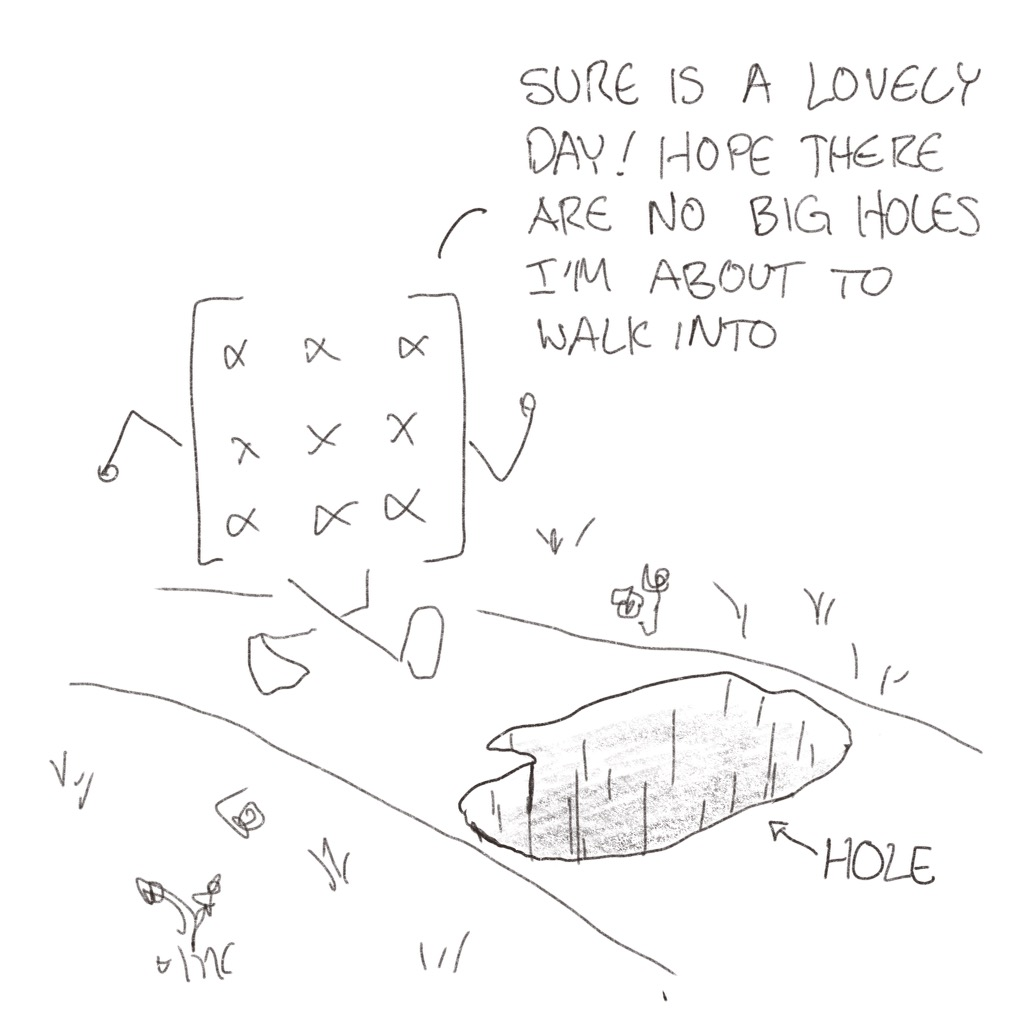
\includegraphics[width=6cm]{gfx/frontart} \\ \medskip

        \mySubtitle \\ \medskip
        %\myDegree \\
        %\myDepartment \\
        %\myFaculty \\
        %\myUni \\ \bigskip

        \myTime\ -- \myVersion

        \vfill

    \end{center}
  \end{addmargin}
\end{titlepage}

%\thispagestyle{empty}

\hfill

\vfill

\noindent\myName: \textit{\myTitle,} \mySubtitle, %\myDegree,
\textcopyright\ \myTime

%\bigskip
%
%\noindent\spacedlowsmallcaps{Supervisors}: \\
%\myProf \\
%\myOtherProf \\
%\mySupervisor
%
%\medskip
%
%\noindent\spacedlowsmallcaps{Location}: \\
%\myLocation
%
%\medskip
%
%\noindent\spacedlowsmallcaps{Time Frame}: \\
%\myTime

\cleardoublepage%*******************************************************
% Dedication
%*******************************************************
\thispagestyle{empty}
\phantomsection
\pdfbookmark[1]{Dedication}{Dedication}

\vspace*{3cm}

\begin{center}
    \emph{Ohana} means family. \\
    Family means nobody gets left behind, or forgotten. \\ \medskip
    --- Lilo \& Stitch
\end{center}

\medskip

\begin{center}
    Dedicated to the loving memory of Rudolf Miede. \\ \smallskip
    1939\,--\,2005
\end{center}

%\cleardoublepage\include{FrontBackmatter/Foreword}
\cleardoublepage%*******************************************************
% Abstract
%*******************************************************
%\renewcommand{\abstractname}{Abstract}
\pdfbookmark[1]{Abstract}{Abstract}
% \addcontentsline{toc}{chapter}{\tocEntry{Abstract}}
\begingroup
\let\clearpage\relax
\let\cleardoublepage\relax
\let\cleardoublepage\relax

\chapter*{Abstract}
A newcomer the greater story of mathematics, free analysis seeks to understand
functions that accept matrices of arbitrary sizes as inputs. Despite the fact
that these functions are naturally noncommutative, many classical results from
the study of complex variables and real algebraic geometry have direct analogues
in this new setting. Unfortunately, the topological underpinnings are still in
flux. In this thesis we cover recent efforts to address these issues---including
the first developments of a theory of algebraic topology of matrix domains.



\vfill
\endgroup

\vfill

%\cleardoublepage%*******************************************************
% Publications
%*******************************************************
\pdfbookmark[1]{Publications}{publications}
\chapter*{Publications}\graffito{This is just an early --~and currently ugly~-- test!}
This might come in handy for PhD theses: some ideas and figures have appeared previously in the following publications:

%\noindent Put your publications from the thesis here. The packages \texttt{multibib} or \texttt{bibtopic} etc. can be used to handle multiple different bibliographies in your document.

\begin{refsection}[ownpubs]
    \small
    \nocite{*} % is local to to the enclosing refsection
    \printbibliography[heading=none]
\end{refsection}

\emph{Attention}: This requires a separate run of \texttt{bibtex} for your \texttt{refsection}, \eg, \texttt{ClassicThesis1-blx} for this file. You might also use \texttt{biber} as the backend for \texttt{biblatex}. See also \url{http://tex.stackexchange.com/questions/128196/problem-with-refsection}.

\cleardoublepage%*******************************************************
% Acknowledgments
%*******************************************************
\pdfbookmark[1]{Acknowledgments}{acknowledgments}

\begin{flushright}{\slshape
    I would contend at all costs both in word and deed\\
    as far as I could that we will be better men, braver\\
    and less idle, if we believe that one must search for \\
    the things one does not know, rather than if we believe \\
    that it is not possible to find out what we do not know \\
    and that we must not look for it.} \\ \medskip
    --- Plato
\end{flushright}



\bigskip

\begingroup
\let\clearpage\relax
\let\cleardoublepage\relax
\let\cleardoublepage\relax
\chapter*{Acknowledgments}

I am deeply indebted to my advisor, Dr.\ Ryan Tully-Doyle, without his firm
push into the world of free analysis this thesis would have never been possible.
I could not have undertaken this journey without Dr.\ Matthew White and Dr.\
Linda Patton. \{A sentence about them\}. To the countless educators who have given their unrelenting
support to my studies, \{the rest of this sentence\}.

\bigskip
I would also like to extend my deepest gratitude to my family. I am who I am
because of your influence---those of you who
have not yet made it to my arm, know that your flower lives in my heart.
I cannot begin to express my thanks to my fellow graduate students. To Karl and
Caroline, thank you for welcoming me into your little family with such open
arms. To Kelsey, for the many late night McDonalds runs. And to Klig, both for
the sandwiches and the conversations.
Finally, I would like to thank Christian Leonard---his contributions to my life
are immeasurable, but by far the greatest is introducing me to H\"aagen-Dazs
Vanilla Swiss Almond.

\endgroup

\cleardoublepage%*******************************************************
% Table of Contents
%*******************************************************
\pagestyle{scrheadings}
%\phantomsection
\pdfbookmark[1]{\contentsname}{tableofcontents}
\setcounter{tocdepth}{2} % <-- 2 includes up to subsections in the ToC
\setcounter{secnumdepth}{3} % <-- 3 numbers up to subsubsections
\manualmark
\markboth{\spacedlowsmallcaps{\contentsname}}{\spacedlowsmallcaps{\contentsname}}
\tableofcontents
\automark[section]{chapter}
\renewcommand{\chaptermark}[1]{\markboth{\spacedlowsmallcaps{#1}}{\spacedlowsmallcaps{#1}}}
\renewcommand{\sectionmark}[1]{\markright{\textsc{\thesection}\enspace\spacedlowsmallcaps{#1}}}
%*******************************************************
% List of Figures and of the Tables
%*******************************************************
\clearpage
% \pagestyle{empty} % Uncomment this line if your lists should not have any headlines with section name and page number
\begingroup
    \let\clearpage\relax
    \let\cleardoublepage\relax
    %*******************************************************
    % List of Figures
    %*******************************************************
    %\phantomsection
    %\addcontentsline{toc}{chapter}{\listfigurename}
    \pdfbookmark[1]{\listfigurename}{lof}
    \listoffigures

    \vspace{8ex}

    %*******************************************************
    % List of Tables
    %*******************************************************
    %\phantomsection
    %\addcontentsline{toc}{chapter}{\listtablename}
    %\pdfbookmark[1]{\listtablename}{lot}
    %\listoftables

    \vspace{8ex}
    % \newpage

    %*******************************************************
    % List of Listings
    %*******************************************************
    %\phantomsection
    %\addcontentsline{toc}{chapter}{\lstlistlistingname}
    %\pdfbookmark[1]{\lstlistlistingname}{lol}
    %\lstlistoflistings

    \vspace{8ex}

    %*******************************************************
    % Acronyms
    %*******************************************************
    %\phantomsection
    %\pdfbookmark[1]{Acronyms}{acronyms}
    %\markboth{\spacedlowsmallcaps{Acronyms}}{\spacedlowsmallcaps{Acronyms}}
    %\chapter*{Acronyms}
    %\begin{acronym}[UMLX]
        %\acro{DRY}{Don't Repeat Yourself}
        %\acro{API}{Application Programming Interface}
        %\acro{UML}{Unified Modeling Language}
    %\end{acronym}

\endgroup

%********************************************************************
% Mainmatter
%*******************************************************
\cleardoublepage
\pagestyle{scrheadings}
\pagenumbering{arabic}
%\setcounter{page}{90}
% use \cleardoublepage here to avoid problems with pdfbookmark
\cleardoublepage
\part{Objects and the Maps Between Them}\label{pt:manual}
%************************************************
\chapter{Introduction}\label{ch:introduction}
%************************************************

\section{Functional Calculus}%
\label{sec:functionalcalc}

Functional Calculus refers to the process of extending the domain of a function
on \(\RR\) to include matrices (or in some cases operators). The most basic
formulation uses the fact that the space \(n \times n\) matrices forms a ring
and so there is a natural way to evaluate polynomials \(f \in \CC [x]\). If we
require that $A \in M_n(\CC)$ is self-adjoint---and hence diagonalizable as
$A = U \Lambda U^*$---then it is a standard result that:
\begin{align*}
  f(A) &= a_nA^n + \cdots + a_1A + a_0 \\
  &= a_n \left( U\Lambda U^* \right) ^n + \cdots + a_1 U\Lambda U^* + a_0 \\
  &= a_n U\Lambda^n U^* + \cdots + a_1 U\Lambda U^* + a_0 \\
  &= U \left( a_n\Lambda ^n + \cdots + a_1\Lambda + a_0 \right) U^* \\
  &= U \left( f(\Lambda) \right) U^*
\end{align*}
Further, since \(\Lambda\) is diagonal and $f$ is a polynomial,
\[
  f \left( \begin{bmatrix} \lambda_1 &  &  \\  & \ddots &  \\  &  & \lambda_n \end{bmatrix}  \right)
  = \begin{bmatrix} f(\lambda_1) &  &  \\  & \ddots &  \\  &  & f(\lambda_n) \end{bmatrix}
\]
Therefore, given a self-adjoint matrix \(A\) and a polynomial \(f \in \CC [x]\)
\[
  f(A) = Uf(\Lambda)U^* = U \;\text{diag}\{f(\lambda_{1}), \dots , f(\lambda_n)\} \; U^*
\]
With this in mind, we can extend a function \(g: [a,b] \to \CC \) to a function
on self adjoint {\color{red} (normal?)} matrices with their spectrum in
\([a,b]\). Let \(A\) be such a matrix (diagonalized by the unitary matrix
\(U\)), and define
\[
  g(A) = U
  \begin{bmatrix} g(\lambda_1) & &\\ &\ddots& \\ & & \lambda_n \end{bmatrix}
  U^*
\]
Thus, for each \(n \in \NN \), \(g\) induces a function on the self-adjoint
\(n \times n\) matrices with spectrum in \([a,b]\).  The natural ordering
{\color{red} {explain why natural?}} on self-adjoint matrices is called the
\textbf{Loewner Order}:

\begin{definition}[Loewner Ordering]
  For like size self-adjoint matrices, we say that \(A \preceq B\) if \(B - A \)
  is positive semidefinite and \(A \prec B\) is \(B-A\) is positive definite.
\end{definition}

With this ordering in place, we can extend many of the familiar function
theoretic properties (monotonicity, convexity) to these matrix-values functions.
In fact, these properties are defined identically to their classical counterpart:
We say that a function is \emph{matrix-monotone} if \(A \preceq B\) implies that
\(f(A) \preceq f(B)\) and \emph{matrix-convex} (or \emph{nc-convex}) if
\[
  f \left( \frac{X+Y}{2} \right) \preceq \frac{f(X)+f(Y)}{2}
\]
for every pair of like-size matrice for which \(f\) is defined. These condition
are rather restrictive (since the must hold for matrices of \emph{all} sizes) so
many functions which are convex/monotone (in the traditional sense) fail to be
matrix-convex/monotone. For example, \(f(x)=x^4\) fails to be nc-convex.
{\color{red} Below is an example from FCAC (Helton). What is the best way to
  refer to this?

Indeed, if
\[
  X = \begin{bmatrix} 4 &2\\2&2 \end{bmatrix}  \qquad \text{ and } \qquad \begin{bmatrix} 2&0\\0&0 \end{bmatrix}
\]
Then
\[
  \frac{X^4+Y^4}{2} - \left( \frac{1}{2}X +\frac{1}{2}Y \right) ^4
  = \begin{bmatrix} 164 &120\\120&84 \end{bmatrix}
\]
Which is not positive definite! Thus \(x^4\) fails to be convex on even
\(2\times 2\) matrices.
}

{\color{blue} nc-positive if positive for all matrices}

Further, a number of the standard constructions lift identically in this
functional calculus.
\begin{definition}[Directional Derivative]
  The derivative of \(f\) in the direction \(H\) is
  \[
    Df(X)[H] = \lim_{t \to 0} \frac{f(X+tH) - f(X)}{t}
  \]
  where \(H\) and \(X\) are like-size self-adjoint matices.
\end{definition}

Often, the best way to compute these directional derivatives is via an
equivalent formulation:
\[
    Df(X)[H] = \left.\frac{df(X+tH)}{dt}\right|_{t=0}
\]
This version allows us to more easily define higher order derivatives
\[
    D^{(k)}f(X)[H] = \left.\frac{d^{(k)}f(X+tH)}{d^{(k)}t}\right|_{t=0}
\]

Despite nc-convexity being so restrictive, Lemma 12 in \cite{heltonFree2013}
shows that the standard characterization of convexity via the second
derivativie: a function \(f\) is convex if and only if \(D^{2}f(X)[H]\) is
nc-positive. Unlike the classical case, however, the only convex polynomials are
of degree 2\footnote{See \cite{heltonFree2013} for details.}.

\section{Extending Multi-Variable Functions}%
\label{sec:ExtMuliVarFun}

We can extend this same functional calculus to functions of several variables,
although the details are a bit more subtle. Let \(x = (x_1 , \dots x_g)\) be a
\(g-tuples\) of noncommuting formal variables and let \(\RR \langle x \rangle\)
{\color{red} why does everyone use \(\RR \) and now \(\CC \)?}
be the ring of nc-polynomials with coefficients in \(\RR \).

{\color{red} Construct the basics and then move on}

\clearpage
%%% Local Variables:
%%% mode: latex
%%% TeX-master: "classicthesis"
%%% End:
\chapter{A Second Attempt}\label{ch:SecondAttempt}

In seeking a more general theory, the functional calculus defined last chapter
is insufficient---it would be useful to be able to define \emph{new} functions
instead of simply lifting polynomials to matrix domains. In a move that will
feel familiar to any good student of mathematics, we will trade treat the
set of self-adjoint matrices and nc polynomials
as prototypical examples of a more general mathematical
object, the so-called \emph{Matrix Universe}.
After defining this new space and the natural maps in
\cref{sec:MatUniv,sec:TracGrad}, we turn our attention to various topologies
places on matrix universes in \cref{sec:TopManUniv}. While the genesis of free
analysis followed \cref{ch:FirstAttempt} (albeit with the usual bumps in the
road that accompany research) modern free analysis looks much more like this
chapter.

\section{Matrix Universes}%
\label{sec:MatUniv}

Beyond the functional calculus, it becomes useful to construct general functions
on spaces of matrices---to do so, we must make this idea of ``spaces of
matrices'' concrete. The largest such space is the so-called \textbf{Matrix
  Universe}---consisting of \(g\)-tuples of matrices of all sizes:
\[
  \MM^g := \bigcup_{n=1}^\infty (M_n(\CC))^g
\]
By convention, when we consider some
\(X = \left( X_1, \dots , X_g \right) \in \MM^g\), we require that the \(X_i\)
are all the same size. Since \(\MM^g\) is such a large set, we often want to
deal with subsets that still carry some of the implicit structure of \(\MM^g\).
\begin{definition}[Free Set]
  \label{def:FreeSet}
  We say \(D \subset \MM^g\) is a \textbf{free set} (also called an nc set) if it is closed with respect
  to direct sums and unitary conjugation. That is
  \begin{enumerate}
    \item \(X,Y \in D \) means \(X\oplus Y \in D\).
    \item For \(X,U\) like-size matrices with \(U\) unitary and \(X \in D\),
          then \(U X U^* = \left( UX_1U^*, \dots , UX_g U^*  \right) \in D \).
  \end{enumerate}
\end{definition}

For the remainder of this text, \(D\) will denote some free set. Using the
terminology of \cite{pascoeFreeNoncommutativePrincipal2020}, let
\(D_n = D \cap M_n(\CC)^g\) be the level-wise slice of all \(n \times n\)
matrices in \(D\). We say that \(D\) is \textbf{nc-open}\footnote{The topology of \(\MM^g\)
  is still in flux and there is not a canonical topology. See section \ref{sec:TopManUniv} for
  the details } (resp.\ \textbf{connected}, \textbf{simply connected}, \textbf{bounded}) if each \(D_n\) is open
(resp.\ connected, simply connected, bounded). Finally, we say that \(D\) is
\textbf{differentiable} if each \(D_n\) is an open \(C^1\) manifold where the
complex tangent space of every \(X \in D_n\) is all of \(M_n(\CC)^g\).
Given some \(X \in \MM^{g} \), there are three associated sets which capture the
structure of free sets.

\begin{definition}[Similarity Envelope]%
\label{def:semenv}
  Given \(X \in \MM^{g} \), a tuple of \(n \times n\) matrices, the
  \textbf{similarity envelope} of \(X\) is the set
  \[
    \{U^* X U \mid  U \in \mathcal{U}_n\}.
  \]
\end{definition}

\begin{definition}[Fiber]%
\label{def:fiber}
  Given \(X \in \MM^{g} \), a tuple of \(n \times n\) matrices, the
  \textbf{fiber} of \(X\) is the set
  \[
    \{X^{\oplus k} \mid  k \in \NN \}.
  \]
\end{definition}

\begin{definition}[Envelope]%
\label{def:env}
  Given \(X \in \MM^{g} \), a tuple of \(n \times n\) matrices, the
  \textbf{envelope} of \(X\) is the set
  \[
    \{ U^* X^{\oplus k} U \mid k \in \NN, U \in \mathcal{U}_{kn} \}.
  \]
\end{definition}
Notice that if \(X \in D\), then the entire envelope of \(X\) is automatically
in \(D\) as well! Further, as shown in example \ref{ex:multivareval},
polynomials respect the envelope of a matrix in a particularly well-behaved way.
Colloquially, we think of all points in the envelope of \(X\) as ``the
same''---this notion is explored in section \ref{sec:TopManUniv} and throughout
chapter \ref{ch:monodromy}.

In the context of \cref{sec:functionalcalc,sec:ExtMuliVarFun}
%
, the domains in the functional calculus were
\(\HH^g = \bigcup_{n=1}^{\infty} {\HH_n}^g\). \(\HH ^g\) is a differentiable, connected
free set.

On \(\MM^{g} \), we define a product that resembles the inner product on
\(\CC^n\) which will be extensively throughout \cref{ch:ZeroDiv,ch:monodromy}.
Given \(A,B \in \MM^{g} \) which are \(g\)-tuples of \(n \times n\) matrices:
\begin{align*}
	\cdot : \MM^{g} \times \MM^{g}  &\longrightarrow M_n(\CC) \\
  \cdot (A,B) = A \cdot B &\longmapsto \sum_{i=1}^g A_i B_i
\end{align*}



\section{Tracial Functions and Uniqueness of the Gradient}%
\label{sec:TracGrad}
Now that we have \(\MM^d\), we can work with general functions on our matrix
universe. As a whole, free analysis is concerned with so-called \emph{free
  functions}, which are graded and
respect direct sums and unitary conjugation.

\begin{definition}[Free Function]
\label{def:FreeFun}
  A function \(f: D\to \MM^{\hat{d}}\) is called \textbf{free} if
  \begin{enumerate}
    \item \(f(X\oplus Y)= f(X) \oplus f(Y)\)
    \item \(f(U X U^*) = f(U)f(X)f(U^*)\) where \(X\) and \(U\) are like-size
          and \(U\) is unitary.
  \end{enumerate}
\end{definition}

The two other classes of functions we are concerned with are those that act like
the trace and the determinant:
\begin{definition}[Determinantal Free Function]%
\label{def:DetFreeFun}
  A function \(f: D \to \CC \) is a \textbf{determinantal free function} if
  \begin{enumerate}
    \item \(f(X\oplus Y) = f(X)f(Y)\)
    \item \(f(U X U^*) = f(X)\) where \(X\) and \(U\) are like-size
          and \(U\) is unitary.
  \end{enumerate}
\end{definition}

\begin{definition}[Tracial Free Function]%
\label{def:TrFreeFun}
  A function \(f: D \to \CC \) is a \textbf{tracial free function} if
  \begin{enumerate}
    \item \(f(X\oplus Y) = f(X)+f(Y)\)
    \item \(f(U X U^*) = f(X)\) where \(X\) and \(U\) are like-size
          and \(U\) is unitary.
  \end{enumerate}
\end{definition}

It is worth noting that, while they share the moniker of \emph{free},
determinantal and tracial functions are \emph{not} free functions.
Since these three classes of functions all contain the word ``free,'' we will
often drop this qualifier and only refer to determinantal, tracial, and free
function.  Given a free function of any type, we can define the directional
derivative (Definition \ref{def:DirDeriv}) identically. It is only these tracial functions which inherit
the gradient mentioned \cref{sec:functionalcalc}.  Similarly to traditional multivariable calculus
we define the gradient via its relationship to the directional derivative:
\begin{definition}[Free Gradient]%
\label{def:FreeGrad}
  Given a tracial free function \(f\), the free gradient, \(\nabla f\), is the
  unique free function satisfying
  \[
    \tr \left( H \cdot \nabla f(X) \right) = \tr\, Df(X)[H]
  \]
\end{definition}

It is not-at-all obvious that such a \(\nabla f \) should be unique---after all
any linear combination of commutator has trace zero. To show the uniqueness of
\(\nabla f\), we will first restrict ourselves to single variable functions. In the case that \(f\)
is a single-variable function we can replace \(\nabla f\) with the traditional
derivative, \(f'\), as seen in
\cite[Thm 3.3]{pascoeTrace2020}.
\begin{theorem}
  Let \(f: (a,b)\to \RR \) be a \(C^1\) function. Then
  \[
    \tr \, Df(X)[H] = \tr \left( Hf'(X) \right)
  \]
\end{theorem}

The proof in \cite{pascoeTrace2020} simply asserts the uniqueness of a function
\(g(X)\) satisfying \(\tr Df(X)[H] = \tr(Hg(X))\) and then shows that
\(g(x)=f'(x)\) for \(x \in (a,b)\). Instead, we can construct such a \(g\) and
recover the theorem along the way:
\begin{proof}

We start with a construction from Bhatia's Matrix Analysis \cite{bhatiaMatrixAnalysis1997}: Let
$f \in C ^{1} (I)$ and define $f ^{[1]} $ on $I \times I$ by
\[
  f^{[1]} (\lambda,\mu) =
  \begin{cases}
    \frac{f(\lambda) - f(\mu)}{\lambda-\mu} & \lambda \neq \mu \\
    f'(\lambda) & \lambda = \mu.
  \end{cases}
\]
We call $f ^{[1]} (\lambda,\mu)$ the \emph{first divided difference} of $f$ at
$(\lambda,\mu)$. If $\Lambda$ is a diagonal matrix with entries
$\{ \lambda_{i}\} $, We may extend $f$ to accept $\Lambda$ by
defining the $(i,j)$-entry of $f ^{[1]} (\Lambda)$ to be
$f ^{[1]} (\lambda_i,\lambda_j)$. If $A$ is a self adjoint matrix with
$A = U \Lambda U ^{*} $, then we define
$f ^{[1]} (A) = U f ^{[1]} (\Lambda) U ^{*} $. Now we borrow a theorem from
Bhatia:
\begin{theorem}[Bhatia V.3.3]
  Let $f \in C ^{1} (I)$ and let $A$ be a self adjoint matrix with all
  eigenvalues in $I$. Then \[
    Df(A)[H] = f ^{[1]} (A) \circ H,
  \]
  where $\circ$ denotes the Schur-product\footnote{Entrywise} in a basis where $A$ is diagonal.
\end{theorem}

That is, if $A = U   \Lambda U ^{*} $, then
\[
  Df(A)[H] = U \left( f ^{[1]} (\Lambda) \circ (U ^{* } H U) \right)U ^{*}.
\]
%
To prove our claim, we need to take the trace of both sides. Since trace is
invariant under a change of basis, it is clear that
\[
  \tr Df(A)[H] = \tr \left( f ^{[1]} (\Lambda) \circ (U ^{* } H U) \right).
\]
If $U = u_{ij}$, $U ^{*} = \overline{u}_{ij}$ and $H = h_{ij}$, then the
$(i,j)$-entry of $U ^{*}HU$ is
\[
  {(U ^{* } H U)}_{ij} = \sum_k\sum_\ell \overline{u}_{ik}h_{k\ell}u_{\ell j}
\]
Where we sum over the duplicate indices $k$ and $\ell$. While the structure of
$f ^{[1]} (\Lambda)$ is a bit unruly, our diagonal entries are $f'(\lambda)$.
This means that when we take the trace of the Schur product, we have
\[
 \sum_k\sum_\ell \sum_i f'(\lambda_i)\overline{u}_{ik}h_{k\ell}u_{\ell i}
\]
Now consider the matrix product
$U\, \text{diag} \{f'(\lambda_1), \dots ,f'(\lambda_n)\} \,U ^{*} H $. Since one of our terms
is diagonal, the trace of this multiplication is simple:
\[
  \text{tr}\; U \,\text{diag} \{f'(\lambda_1), \dots ,f'(\lambda_n)\}\, U ^{*} H
  = \sum_k\sum_\ell\sum_i  u_{ik}f'(\lambda_k) \overline{u}_{k \ell} h_{\ell i}
\]
Since \(u_{ik}, \overline{u}_{k\ell}, h_{\ell i} \in \CC \) they commute. We can
then relabel our indices
$i \mapsto \ell\; \ell \mapsto k \; k \mapsto i $ to get
\[
  \tr\; U \,\text{diag} \{f'(\lambda_1), \dots ,f'(\lambda_n)\}\, U ^{*} H
  = \sum_k\sum_\ell \sum_i f'(\lambda_i) \overline{u}_{i k} h_{k \ell}u_{\ell i},
\]
So, for every direction \(H\), we have that
\[
  \tr \left( U\, \text{diag} \{f'(\lambda_1), \dots ,f'(\lambda_n)\} \,U ^{*} H\right) =
  \tr \left( f ^{[1]} (\Lambda) \circ (U ^{* } H U) \right).
\]
By picking the ``correct'' \(H\),
\footnote{See the proof of \ref{thm:trdual} for the details of how to pick the
  \(H\)'s}
we conclude that there is a unique quantity \(g(X)\) satisfying
\[
  \tr \;Df(X)[H] = \tr(Hg(X)).
\]
In particular,
\( g(X) = U\, \text{diag} \{f'(\lambda_1), \dots ,f'(\lambda_n)\} \,U ^{*} \). But,
recall that \(X=U\Lambda U\) so, in the functional calculus, $g(X) = f'(X)$.
Making this substitution, we have the required result:
\[
  \tr \; Df(X)[H] = \tr (H f'(X))
\]
\end{proof}

With our theorem proven, we turn our attention back to the \(\nabla f\). The
single variable case motivates that \(\nabla f\) should correspond to the
standard gradient from vector calculus. With some work, the above proof lifts
the multi-variable case. It will be instructive, however, to consider a
different proof.

\begin{theorem}[Trace Duality]%
\label{thm:trdual}
Let \(f,g\) be free functions \(\MM^{g} \to \MM^{\tilde{g}} \). If
\(\tr H \cdot f = \tr H \cdot g\) for all tuples \(H\), then \(f=g\).
\end{theorem}

\begin{proof}
  Since the trace relation holds for all $H$, we may choose our $H$ carefully to
  show the equality of $f$ and $g$. Say that $H,f(X),g(X)$ are $g$-tuples of
  matrices---we will first show that $f_1=g_1$ and we will do so entry by entry.
  Let $E_{ij}$ be the matrix will all zeroes and a \(1\) in the $(i,j)$-entry.  Now
  let $H= (E_{ji},0, \dots ,0)$. So $\tr E_{ji}f_1(X) = \tr E_{ji}g_1(X)$.
  In our products, the only elements on the diagonal are $(f_1(X))_{ij}$ and
  $(g_1(X))_{ij}$, so when we take the trace we have $(f_1(X))_{ij} =(g_1(X))_{ij}$. If we
  do this for every $(i,j)$, we see that $f_1(X)=g_1(X)$. Similarly, we can choose
  \(H = ( 0, E_{ji},0, \dots, 0)\) for each \(i,j\) to show that \(f_2(X)=g_2(X)\) and
  so on. Since \(f(X)=g(X)\) for each \(X \in \MM^{g} \), it follows that \(f=g\).
\end{proof}

Admittedly, there is a slight complication that is overlooked in the above proof
when it comes to the domains of \(f\) and \(g\). Where these domains overlap, we
can consider them as the same function (and therefore \(\nabla f \) is unique)
but if \(f\) is defined on \(D\) and \(g\) is defined on \(\tilde{D}\), then the
above proof only holds on \(D \cap \tilde{D}\). This complication  occurs
semi-frequently in free analysis, but in generally swept under the rug---if two
free functions agree the intersection of their domains, it is convention to
consider them equivalent. Examples
of such \(f\) and \(g\) abound when considering rational functions, which are
explored in \cref{sec:ncrational}.

\section{The Topology of Matrix Universes }%
\label{sec:TopManUniv}

At the time of writing, there is no ``canonical topology'' for \(\MM^g\). For a
long time it seemed like the \emph{free} topology (to be defined below) was the
obvious choice, but recent work (c.f.\ \cite{pascoeentire2019}) has implied that the free
topology does not put enough structure on \(\MM^g\). See \cite{aglerAspects2016}
for a full treatment of the common topologies on \(\MM^g\).

A naive approach to a topology on \(\MM = \bigcup_n M_n(\CC)\) would be the
disjoint union topology---which is then extended do a topology on \(\MM^g\) via
the product topology. Notice, however that this ignores a significant amount of
the implicit structure of nc sets as we get a disconnected space with countable
many connected components. Topologically, this is means that means that
\[
  H_\bullet (D) = \bigoplus_{n \in \NN } H_\bullet(D_n).
\]
At first glance, this seems fine enough, but it ignores the fact that for
\(X \in D\) we require \(X^{\oplus k} \in D\) for all \(k\) and \(U^*XU \in D\)
for all unitary \(U\). In a sense, we think of the all the direct sums of \(X\)
and its similarity envelope as ``the same.'' In light of this, if \(\sim\) is
the equivalence relation that \(X\sim Y\) if \(Y = X^{\oplus k}\) or
\(Y = U^*XU\) ,
then any useful topological theory on \(D \subset \MM^g\) should descend to
classic theory on \(\faktor{D}{\sim}\). One needs only look at \(H_0(D)\) to see
that the naive approach fails to give useful information. It should be the case
that \(H_0(\MM^{g} )\) is trivial but in the disjoint union topology it is easy
to see
\[
  H_0(\MM^{g} ) = \bigoplus_{n \in \NN } \ZZ ,
\]
which does not behave as we would expect.


\subsection{Admissible Topologies}%
\label{sec:admtopo}

{\color{blue} a cool example is showing that \(\HH \) is dense in \(\MM\)? It
  would be good to see the level-wise-ness of the fine topology but it is not
  difficult.}

In light of the above discussion, we will present some of the candidate
topologies which show some promise in understanding the topology on \(\MM^g\)
and its subsets.
Let \(D \subset \MM^{g} \) be a nc bounded open set (recall that this means that \(D\) is closed under
direct sums and unitary conjugation, and that each \(D_n\) is a bounded open set
in \(M_n(\CC)^g\)) and let
\[
  \mathcal{B} = \{D \mid  D \textrm{ is an nc bounded open set}\} .
\]
It is not difficult to se that \(\mathcal{B}\) is the basis for a topology on
\(\MM^{g}\), called the \textbf{fine} topology. Currently, there is not a
``standard'' topology for \(\MM^{g}\). Any topology on, \(\tau\), \(\MM^{g}\) is
considered \textbf{admissable} if it basis is a subset of \(\mathcal{B}\)---\ie
it has a basis of nc bounded open sets.

A slightly more restrictive topology (that seems to show some promise in the eyes
of the author) is the \textbf{fat} topology. For \(n \in \NN \),
\(r \in \RR ^+\), and \(X \in \MM^g_n\), we first define a matricial polydisc
\[
  D_n(X,r) := \{A \in \MM^g \mid \max_{1\leq i\leq g} \| X_i-A_i \| <r\}.
\]
Now we sweep \(D_n\) through all direct sum copies of \(X\):
\[
  D(X,r) := \bigcup_{k=1}^\infty D_{kn} (X^{\oplus k},r)
\]
Finally, we take the similarity envelope of \(D(X,r)\)
\[
  F(X,r) :=  \bigcup_{n=1}^\infty \bigcup_{U \in \mathcal{U}_n} U^* \left( D(X,r) \cap \MM^g_n \right) U
\]
Both the fine and the fat topologies admit implicit function theorems---which
are discussed (in brief) in \cref{sec:freeanal}.

The final candidate topology is the aforementioned \textbf{free} topology.
Recall that \(\RR \langle x \rangle \) is the algebra of nc polynomials over the
real numbers and that
\(\RR \langle x \rangle ^{k\times k}\) is the set of \(k \times k\) matrices
with entries in \(\RR \langle x \rangle \). Let
\(\delta \in \RR \langle x \rangle ^{k\times k}\) and define
\[
  G_\delta = \{x \in \MM^{g} \mid \| \delta(x) \| <1\}.
\]
For \(x \in M_n(\CC)\), \(\|\cdot \|\) is the operator norm in
\(\mathcal{B}(\CC^k\otimes\CC^n)\). This may seem strange
\footnote{The author would like to note that it is, in fact, strange.}
but the level-wise definition allows the norm to ``play nice'' with direct sums.
The set of all \(G_\delta\) as \(k\) ranges over \(\ZZ ^+\) form the basis for
the free topology. Indeed, any \(X \in \MM^{g} \) is trivially in one of the
\(G_\delta\) (take \(\delta=X\)) and with some work one can show that
\(G_{\delta_1} \cap G_{\delta_2}= G_{\delta_1\oplus \delta_2}\) so we do,
indeed, have a basis. All that is needed to satisfy the axioms for a base is that
\(G_{\delta_1} \cap G_{\delta_2} \supset G_{\delta_1\oplus \delta_2}\). In
fact if one chose a more ``standard'' norm for \(\delta(X)\) above (\eg the
Frobenius norm) one gets the needed inclusion. The benefit of the strange norm,
however, is that we get equality here instead of inclusion.

\section{Free Analogues of Classical Results}%
\label{sec:freeanal}

In general, efforts to reprove classical results from single and several varible
complex analysis have been successful. A full treatise of the results proven
before 2020 can be found in \cite{aglerOperator2019}---but we will include a
handful here.

Among the many astounding results is the following characterization of
holomorphic functions in admissible topologies:
\begin{theorem}[Locally Bounded Implies Analytic]
  Let \(D\) be an nc domain and \(f\) a free function on \(D\). If \(f\) is
  locally bounded on each \(D_n\), then \(f\) is an analytic function of the
  entries of the matrices at each level \(n\).
\end{theorem}
A proof for this (rather suprising) result is given in \cite{heltonProper2011}.
With different topologies come different analytic functions. In light of this,
if the topology is not understood functions are usually referred to as
\{fine/fat/free\} holomorphic.
As mentioned above, both the fine and fat topologies have implicit function
theorems. The fat implicit function theorem requires a significant amount more
work to state, but it can be found in \cite{aglerOperator2019}.
\begin{theorem}[Fine Implicit Function Theorem]
  Let \(D \subset \MM^g\) be an nc domain. Let \(\Phi\) be a fine holomorphic
  map \(D\to \MM^{g} \). The following equivalent:
  \begin{enumerate}
    \item \(\Phi\) is injective on \(D\)
    \item \(D\Phi(X)[H]\) is nonsingular for every \(X \in D\) and like-size
          \(H \in \MM^{g}\).
    \item the function \(\Phi ^{-1}\) exists and is a fine holomorphic
          map.
  \end{enumerate}
\end{theorem}

Various Null- and Positivstellensatz
\footnote{And even a QuadratischePositivstellensatz!} exist throughout the
literature extending Hilbert's famous Nullstellensatz in algebraic
geometry---many of which utilize the idea of so-called ``atomic'' matrices of nc
polynomials (defined in \cref{def:atomic}). See \cite{heltonFactorization2019}
for the specifics.

In \cite{aglerGlobal2013}, Agler and McCarthy prove a free analogue of the
Oka-Weil theorem: any free holomorphic function on a compact set
can be uniformly approximated by polynomials. Unfortunately, it was later proven
in \cite{pascoeInvariant2021} and \cite{augatCompact2017} that the only compact
sets in the \(\MM^{g} \) are the envelope of finitely many points, trivializing
the result of Agler and McCarthy.


{\color{fgreen} This section feels very out of place but I'm not sure where it
  should go}
For the rest of this thesis, we will be using the conventions mentioned in
\cref{sec:MatUniv}: \( D \subset\MM^{g} \) open if each \(D_n\) is open---these
are precisely the basic open sets in the fine topology.
Given \(X,Y \in D\), it is not generally true that we can separate \(X\) and
\(Y\) with open sets. However if \(Y\) is not in the similarity envelope of
\(X\) and \(X\) and \(Y\) have disjoint fibers, then we \emph{can} separate
them! Motivated by definitions in section \ref{sec:trpi1} we call a topology
satisfying this condition (Hausdorff outside of the similarity envelope and
fiber) \textbf{essentially Hausdorff}.


\section{nc Rational Functions}%
\label{sec:ncrational}

While polynomials were fairly simply to lift to the noncommutative setting,
dealing with rational functions is a bit more complex. In depth discussion of nc
rational functions descends quickly into abstract nonsense, so we will only
cover the basics and will not go beyond what is needed for the work done in the
rest of this thesis.

\begin{definition}[nc Rational Expression]%
\label{def:ratexp}
  An \textbf{nc rational expression} (alternativey a free rational expression)
  in noncommuting indeterminants, \(x_1, \dots ,x_g\) is a syntactically valid
  expression of those indeterminants involving addition, multiplicatoin, inverses,
  and scalar multiplication.
\end{definition}

For example, the following are examples of free rational expressions in two
variables:
\begin{equation*}
\begin{split}
  x_1x_2+x_2x_1(x_1-x_2)^{-1} &,\; (2x_2^2x_1^{-1} +(x_1x_2-x_2x_1)^{-1}) ,\\
 (x_2(1-x_1x_2)&-(1-x_2x_1)x_2)^{-1}.
\end{split}
\end{equation*}

The careful reader will notice, however, that one of these expressions is not
like the other. If we were to evaluate these expression on tuples of matrices,
there is no pair for which \((x_2(1-x_1x_2)-(1-x_2x_1)x_2)^{-1}\) is defined.
This is an example of a \textbf{degenerate} rational expression. Formally, an nc
rational expression is \textbf{nondegenerate} if there is at least one
\(X \in \MM^{g} \) such that \(r(X)\) is defined.

When seeking to make rational \emph{functions} out of a nondegenerate rational
expression, one encounters significant difficulties. For example,
\[
  x_1-x_1+x_2 ^{-1} x_2-1 \quad \textrm{ and } \quad 0
\]
are syntactically distinct nc rational expressions, have wildly different
domains, yet whenever their domains of evaluation align, they will give the
same evaluation.  With the likes of the Identity Theorem from complex analysis
one would like to say that these are the same function. In light of this, nc
rational functions are defined via equivalence classes. We say two rational
expressions, \(r_1,r_2\), are equivalent if \(r_1(X) = r_2(X)\) whenever both
expressions are defined.

Unforunately, this introduces a new wrinkle. There is, of course, the issue of
what the domain of the equivalence class is---usually one simply works with the
domain of the representative chosen. Moreover, given two representatives of the
same equivalence class of rational functions, there is no guarantee of an
algebraic manipulation to transform one into the other.

Just like the polynomial case, we often consider \emph{matrices} of nc rational
functions. Chapter \ref{ch:ZeroDiv} explores the algebraic geometry of nc
polynomials and rational functions. Thankfully, however, we do not
need any of the in depth theory of rational functions. \cite{heltonFree2013}
contains a slightly broader introduction from an analytical lens while \cite{cohnFree2006}
provides a (more complete) algebraic treatment. The only theorem we will need
comes from the latter:

\begin{theorem}
\label{thm:ratchar}
  For any nondegenerate
  rational expression, \(r\), there is a linear square matrix of polynomials, \(L\), and
  rectangular constants \(b,c\) such that \(r=b^*L ^{-1}c\)---where \(L ^{-1}\) is
  defined wherever \(r\) is defined.
\end{theorem}

\cleardoublepage
\ctparttext{You can put some informational part preamble text here.
Illo principalmente su nos. Non message \emph{occidental} angloromanic
da. Debitas effortio simplificate sia se, auxiliar summarios da que,
se avantiate publicationes via. Pan in terra summarios, capital
interlingua se que. Al via multo esser specimen, campo responder que
da. Le usate medical addresses pro, europa origine sanctificate nos se.}
\part{The Showcase}\label{pt:showcase}
%%%% Local Variables:
%%% mode: latex
%%% TeX-master: "classicthesis"
%%% End:
\chapter{A Second Attempt}\label{ch:SecondAttempt}

In seeking a more general theory, the functional calculus defined last chapter
is insufficient---it would be useful to be able to define \emph{new} functions
instead of simply lifting polynomials to matrix domains. In a move that will
feel familiar to any good student of mathematics, we will trade treat the
set of self-adjoint matrices and nc polynomials
as prototypical examples of a more general mathematical
object, the so-called \emph{Matrix Universe}.
After defining this new space and the natural maps in
\cref{sec:MatUniv,sec:TracGrad}, we turn our attention to various topologies
places on matrix universes in \cref{sec:TopManUniv}. While the genesis of free
analysis followed \cref{ch:FirstAttempt} (albeit with the usual bumps in the
road that accompany research) modern free analysis looks much more like this
chapter.

\section{Matrix Universes}%
\label{sec:MatUniv}

Beyond the functional calculus, it becomes useful to construct general functions
on spaces of matrices---to do so, we must make this idea of ``spaces of
matrices'' concrete. The largest such space is the so-called \textbf{Matrix
  Universe}---consisting of \(g\)-tuples of matrices of all sizes:
\[
  \MM^g := \bigcup_{n=1}^\infty (M_n(\CC))^g
\]
By convention, when we consider some
\(X = \left( X_1, \dots , X_g \right) \in \MM^g\), we require that the \(X_i\)
are all the same size. Since \(\MM^g\) is such a large set, we often want to
deal with subsets that still carry some of the implicit structure of \(\MM^g\).
\begin{definition}[Free Set]
  \label{def:FreeSet}
  We say \(D \subset \MM^g\) is a \textbf{free set} (also called an nc set) if it is closed with respect
  to direct sums and unitary conjugation. That is
  \begin{enumerate}
    \item \(X,Y \in D \) means \(X\oplus Y \in D\).
    \item For \(X,U\) like-size matrices with \(U\) unitary and \(X \in D\),
          then \(U X U^* = \left( UX_1U^*, \dots , UX_g U^*  \right) \in D \).
  \end{enumerate}
\end{definition}

For the remainder of this text, \(D\) will denote some free set. Using the
terminology of \cite{pascoeFreeNoncommutativePrincipal2020}, let
\(D_n = D \cap M_n(\CC)^g\) be the level-wise slice of all \(n \times n\)
matrices in \(D\). We say that \(D\) is \textbf{nc-open}\footnote{The topology of \(\MM^g\)
  is still in flux and there is not a canonical topology. See section \ref{sec:TopManUniv} for
  the details } (resp.\ \textbf{connected}, \textbf{simply connected}, \textbf{bounded}) if each \(D_n\) is open
(resp.\ connected, simply connected, bounded). Finally, we say that \(D\) is
\textbf{differentiable} if each \(D_n\) is an open \(C^1\) manifold where the
complex tangent space of every \(X \in D_n\) is all of \(M_n(\CC)^g\).
Given some \(X \in \MM^{g} \), there are three associated sets which capture the
structure of free sets.

\begin{definition}[Similarity Envelope]%
\label{def:semenv}
  Given \(X \in \MM^{g} \), a tuple of \(n \times n\) matrices, the
  \textbf{similarity envelope} of \(X\) is the set
  \[
    \{U^* X U \mid  U \in \mathcal{U}_n\}.
  \]
\end{definition}

\begin{definition}[Fiber]%
\label{def:fiber}
  Given \(X \in \MM^{g} \), a tuple of \(n \times n\) matrices, the
  \textbf{fiber} of \(X\) is the set
  \[
    \{X^{\oplus k} \mid  k \in \NN \}.
  \]
\end{definition}

\begin{definition}[Envelope]%
\label{def:env}
  Given \(X \in \MM^{g} \), a tuple of \(n \times n\) matrices, the
  \textbf{envelope} of \(X\) is the set
  \[
    \{ U^* X^{\oplus k} U \mid k \in \NN, U \in \mathcal{U}_{kn} \}.
  \]
\end{definition}
Notice that if \(X \in D\), then the entire envelope of \(X\) is automatically
in \(D\) as well! Further, as shown in example \ref{ex:multivareval},
polynomials respect the envelope of a matrix in a particularly well-behaved way.
Colloquially, we think of all points in the envelope of \(X\) as ``the
same''---this notion is explored in section \ref{sec:TopManUniv} and throughout
chapter \ref{ch:monodromy}.

In the context of \cref{sec:functionalcalc,sec:ExtMuliVarFun}
%
, the domains in the functional calculus were
\(\HH^g = \bigcup_{n=1}^{\infty} {\HH_n}^g\). \(\HH ^g\) is a differentiable, connected
free set.

On \(\MM^{g} \), we define a product that resembles the inner product on
\(\CC^n\) which will be extensively throughout \cref{ch:ZeroDiv,ch:monodromy}.
Given \(A,B \in \MM^{g} \) which are \(g\)-tuples of \(n \times n\) matrices:
\begin{align*}
	\cdot : \MM^{g} \times \MM^{g}  &\longrightarrow M_n(\CC) \\
  \cdot (A,B) = A \cdot B &\longmapsto \sum_{i=1}^g A_i B_i
\end{align*}



\section{Tracial Functions and Uniqueness of the Gradient}%
\label{sec:TracGrad}
Now that we have \(\MM^d\), we can work with general functions on our matrix
universe. As a whole, free analysis is concerned with so-called \emph{free
  functions}, which are graded and
respect direct sums and unitary conjugation.

\begin{definition}[Free Function]
\label{def:FreeFun}
  A function \(f: D\to \MM^{\hat{d}}\) is called \textbf{free} if
  \begin{enumerate}
    \item \(f(X\oplus Y)= f(X) \oplus f(Y)\)
    \item \(f(U X U^*) = f(U)f(X)f(U^*)\) where \(X\) and \(U\) are like-size
          and \(U\) is unitary.
  \end{enumerate}
\end{definition}

The two other classes of functions we are concerned with are those that act like
the trace and the determinant:
\begin{definition}[Determinantal Free Function]%
\label{def:DetFreeFun}
  A function \(f: D \to \CC \) is a \textbf{determinantal free function} if
  \begin{enumerate}
    \item \(f(X\oplus Y) = f(X)f(Y)\)
    \item \(f(U X U^*) = f(X)\) where \(X\) and \(U\) are like-size
          and \(U\) is unitary.
  \end{enumerate}
\end{definition}

\begin{definition}[Tracial Free Function]%
\label{def:TrFreeFun}
  A function \(f: D \to \CC \) is a \textbf{tracial free function} if
  \begin{enumerate}
    \item \(f(X\oplus Y) = f(X)+f(Y)\)
    \item \(f(U X U^*) = f(X)\) where \(X\) and \(U\) are like-size
          and \(U\) is unitary.
  \end{enumerate}
\end{definition}

It is worth noting that, while they share the moniker of \emph{free},
determinantal and tracial functions are \emph{not} free functions.
Since these three classes of functions all contain the word ``free,'' we will
often drop this qualifier and only refer to determinantal, tracial, and free
function.  Given a free function of any type, we can define the directional
derivative (Definition \ref{def:DirDeriv}) identically. It is only these tracial functions which inherit
the gradient mentioned \cref{sec:functionalcalc}.  Similarly to traditional multivariable calculus
we define the gradient via its relationship to the directional derivative:
\begin{definition}[Free Gradient]%
\label{def:FreeGrad}
  Given a tracial free function \(f\), the free gradient, \(\nabla f\), is the
  unique free function satisfying
  \[
    \tr \left( H \cdot \nabla f(X) \right) = \tr\, Df(X)[H]
  \]
\end{definition}

It is not-at-all obvious that such a \(\nabla f \) should be unique---after all
any linear combination of commutator has trace zero. To show the uniqueness of
\(\nabla f\), we will first restrict ourselves to single variable functions. In the case that \(f\)
is a single-variable function we can replace \(\nabla f\) with the traditional
derivative, \(f'\), as seen in
\cite[Thm 3.3]{pascoeTrace2020}.
\begin{theorem}
  Let \(f: (a,b)\to \RR \) be a \(C^1\) function. Then
  \[
    \tr \, Df(X)[H] = \tr \left( Hf'(X) \right)
  \]
\end{theorem}

The proof in \cite{pascoeTrace2020} simply asserts the uniqueness of a function
\(g(X)\) satisfying \(\tr Df(X)[H] = \tr(Hg(X))\) and then shows that
\(g(x)=f'(x)\) for \(x \in (a,b)\). Instead, we can construct such a \(g\) and
recover the theorem along the way:
\begin{proof}

We start with a construction from Bhatia's Matrix Analysis \cite{bhatiaMatrixAnalysis1997}: Let
$f \in C ^{1} (I)$ and define $f ^{[1]} $ on $I \times I$ by
\[
  f^{[1]} (\lambda,\mu) =
  \begin{cases}
    \frac{f(\lambda) - f(\mu)}{\lambda-\mu} & \lambda \neq \mu \\
    f'(\lambda) & \lambda = \mu.
  \end{cases}
\]
We call $f ^{[1]} (\lambda,\mu)$ the \emph{first divided difference} of $f$ at
$(\lambda,\mu)$. If $\Lambda$ is a diagonal matrix with entries
$\{ \lambda_{i}\} $, We may extend $f$ to accept $\Lambda$ by
defining the $(i,j)$-entry of $f ^{[1]} (\Lambda)$ to be
$f ^{[1]} (\lambda_i,\lambda_j)$. If $A$ is a self adjoint matrix with
$A = U \Lambda U ^{*} $, then we define
$f ^{[1]} (A) = U f ^{[1]} (\Lambda) U ^{*} $. Now we borrow a theorem from
Bhatia:
\begin{theorem}[Bhatia V.3.3]
  Let $f \in C ^{1} (I)$ and let $A$ be a self adjoint matrix with all
  eigenvalues in $I$. Then \[
    Df(A)[H] = f ^{[1]} (A) \circ H,
  \]
  where $\circ$ denotes the Schur-product\footnote{Entrywise} in a basis where $A$ is diagonal.
\end{theorem}

That is, if $A = U   \Lambda U ^{*} $, then
\[
  Df(A)[H] = U \left( f ^{[1]} (\Lambda) \circ (U ^{* } H U) \right)U ^{*}.
\]
%
To prove our claim, we need to take the trace of both sides. Since trace is
invariant under a change of basis, it is clear that
\[
  \tr Df(A)[H] = \tr \left( f ^{[1]} (\Lambda) \circ (U ^{* } H U) \right).
\]
If $U = u_{ij}$, $U ^{*} = \overline{u}_{ij}$ and $H = h_{ij}$, then the
$(i,j)$-entry of $U ^{*}HU$ is
\[
  {(U ^{* } H U)}_{ij} = \sum_k\sum_\ell \overline{u}_{ik}h_{k\ell}u_{\ell j}
\]
Where we sum over the duplicate indices $k$ and $\ell$. While the structure of
$f ^{[1]} (\Lambda)$ is a bit unruly, our diagonal entries are $f'(\lambda)$.
This means that when we take the trace of the Schur product, we have
\[
 \sum_k\sum_\ell \sum_i f'(\lambda_i)\overline{u}_{ik}h_{k\ell}u_{\ell i}
\]
Now consider the matrix product
$U\, \text{diag} \{f'(\lambda_1), \dots ,f'(\lambda_n)\} \,U ^{*} H $. Since one of our terms
is diagonal, the trace of this multiplication is simple:
\[
  \text{tr}\; U \,\text{diag} \{f'(\lambda_1), \dots ,f'(\lambda_n)\}\, U ^{*} H
  = \sum_k\sum_\ell\sum_i  u_{ik}f'(\lambda_k) \overline{u}_{k \ell} h_{\ell i}
\]
Since \(u_{ik}, \overline{u}_{k\ell}, h_{\ell i} \in \CC \) they commute. We can
then relabel our indices
$i \mapsto \ell\; \ell \mapsto k \; k \mapsto i $ to get
\[
  \tr\; U \,\text{diag} \{f'(\lambda_1), \dots ,f'(\lambda_n)\}\, U ^{*} H
  = \sum_k\sum_\ell \sum_i f'(\lambda_i) \overline{u}_{i k} h_{k \ell}u_{\ell i},
\]
So, for every direction \(H\), we have that
\[
  \tr \left( U\, \text{diag} \{f'(\lambda_1), \dots ,f'(\lambda_n)\} \,U ^{*} H\right) =
  \tr \left( f ^{[1]} (\Lambda) \circ (U ^{* } H U) \right).
\]
By picking the ``correct'' \(H\),
\footnote{See the proof of \ref{thm:trdual} for the details of how to pick the
  \(H\)'s}
we conclude that there is a unique quantity \(g(X)\) satisfying
\[
  \tr \;Df(X)[H] = \tr(Hg(X)).
\]
In particular,
\( g(X) = U\, \text{diag} \{f'(\lambda_1), \dots ,f'(\lambda_n)\} \,U ^{*} \). But,
recall that \(X=U\Lambda U\) so, in the functional calculus, $g(X) = f'(X)$.
Making this substitution, we have the required result:
\[
  \tr \; Df(X)[H] = \tr (H f'(X))
\]
\end{proof}

With our theorem proven, we turn our attention back to the \(\nabla f\). The
single variable case motivates that \(\nabla f\) should correspond to the
standard gradient from vector calculus. With some work, the above proof lifts
the multi-variable case. It will be instructive, however, to consider a
different proof.

\begin{theorem}[Trace Duality]%
\label{thm:trdual}
Let \(f,g\) be free functions \(\MM^{g} \to \MM^{\tilde{g}} \). If
\(\tr H \cdot f = \tr H \cdot g\) for all tuples \(H\), then \(f=g\).
\end{theorem}

\begin{proof}
  Since the trace relation holds for all $H$, we may choose our $H$ carefully to
  show the equality of $f$ and $g$. Say that $H,f(X),g(X)$ are $g$-tuples of
  matrices---we will first show that $f_1=g_1$ and we will do so entry by entry.
  Let $E_{ij}$ be the matrix will all zeroes and a \(1\) in the $(i,j)$-entry.  Now
  let $H= (E_{ji},0, \dots ,0)$. So $\tr E_{ji}f_1(X) = \tr E_{ji}g_1(X)$.
  In our products, the only elements on the diagonal are $(f_1(X))_{ij}$ and
  $(g_1(X))_{ij}$, so when we take the trace we have $(f_1(X))_{ij} =(g_1(X))_{ij}$. If we
  do this for every $(i,j)$, we see that $f_1(X)=g_1(X)$. Similarly, we can choose
  \(H = ( 0, E_{ji},0, \dots, 0)\) for each \(i,j\) to show that \(f_2(X)=g_2(X)\) and
  so on. Since \(f(X)=g(X)\) for each \(X \in \MM^{g} \), it follows that \(f=g\).
\end{proof}

Admittedly, there is a slight complication that is overlooked in the above proof
when it comes to the domains of \(f\) and \(g\). Where these domains overlap, we
can consider them as the same function (and therefore \(\nabla f \) is unique)
but if \(f\) is defined on \(D\) and \(g\) is defined on \(\tilde{D}\), then the
above proof only holds on \(D \cap \tilde{D}\). This complication  occurs
semi-frequently in free analysis, but in generally swept under the rug---if two
free functions agree the intersection of their domains, it is convention to
consider them equivalent. Examples
of such \(f\) and \(g\) abound when considering rational functions, which are
explored in \cref{sec:ncrational}.

\section{The Topology of Matrix Universes }%
\label{sec:TopManUniv}

At the time of writing, there is no ``canonical topology'' for \(\MM^g\). For a
long time it seemed like the \emph{free} topology (to be defined below) was the
obvious choice, but recent work (c.f.\ \cite{pascoeentire2019}) has implied that the free
topology does not put enough structure on \(\MM^g\). See \cite{aglerAspects2016}
for a full treatment of the common topologies on \(\MM^g\).

A naive approach to a topology on \(\MM = \bigcup_n M_n(\CC)\) would be the
disjoint union topology---which is then extended do a topology on \(\MM^g\) via
the product topology. Notice, however that this ignores a significant amount of
the implicit structure of nc sets as we get a disconnected space with countable
many connected components. Topologically, this is means that means that
\[
  H_\bullet (D) = \bigoplus_{n \in \NN } H_\bullet(D_n).
\]
At first glance, this seems fine enough, but it ignores the fact that for
\(X \in D\) we require \(X^{\oplus k} \in D\) for all \(k\) and \(U^*XU \in D\)
for all unitary \(U\). In a sense, we think of the all the direct sums of \(X\)
and its similarity envelope as ``the same.'' In light of this, if \(\sim\) is
the equivalence relation that \(X\sim Y\) if \(Y = X^{\oplus k}\) or
\(Y = U^*XU\) ,
then any useful topological theory on \(D \subset \MM^g\) should descend to
classic theory on \(\faktor{D}{\sim}\). One needs only look at \(H_0(D)\) to see
that the naive approach fails to give useful information. It should be the case
that \(H_0(\MM^{g} )\) is trivial but in the disjoint union topology it is easy
to see
\[
  H_0(\MM^{g} ) = \bigoplus_{n \in \NN } \ZZ ,
\]
which does not behave as we would expect.


\subsection{Admissible Topologies}%
\label{sec:admtopo}

{\color{blue} a cool example is showing that \(\HH \) is dense in \(\MM\)? It
  would be good to see the level-wise-ness of the fine topology but it is not
  difficult.}

In light of the above discussion, we will present some of the candidate
topologies which show some promise in understanding the topology on \(\MM^g\)
and its subsets.
Let \(D \subset \MM^{g} \) be a nc bounded open set (recall that this means that \(D\) is closed under
direct sums and unitary conjugation, and that each \(D_n\) is a bounded open set
in \(M_n(\CC)^g\)) and let
\[
  \mathcal{B} = \{D \mid  D \textrm{ is an nc bounded open set}\} .
\]
It is not difficult to se that \(\mathcal{B}\) is the basis for a topology on
\(\MM^{g}\), called the \textbf{fine} topology. Currently, there is not a
``standard'' topology for \(\MM^{g}\). Any topology on, \(\tau\), \(\MM^{g}\) is
considered \textbf{admissable} if it basis is a subset of \(\mathcal{B}\)---\ie
it has a basis of nc bounded open sets.

A slightly more restrictive topology (that seems to show some promise in the eyes
of the author) is the \textbf{fat} topology. For \(n \in \NN \),
\(r \in \RR ^+\), and \(X \in \MM^g_n\), we first define a matricial polydisc
\[
  D_n(X,r) := \{A \in \MM^g \mid \max_{1\leq i\leq g} \| X_i-A_i \| <r\}.
\]
Now we sweep \(D_n\) through all direct sum copies of \(X\):
\[
  D(X,r) := \bigcup_{k=1}^\infty D_{kn} (X^{\oplus k},r)
\]
Finally, we take the similarity envelope of \(D(X,r)\)
\[
  F(X,r) :=  \bigcup_{n=1}^\infty \bigcup_{U \in \mathcal{U}_n} U^* \left( D(X,r) \cap \MM^g_n \right) U
\]
Both the fine and the fat topologies admit implicit function theorems---which
are discussed (in brief) in \cref{sec:freeanal}.

The final candidate topology is the aforementioned \textbf{free} topology.
Recall that \(\RR \langle x \rangle \) is the algebra of nc polynomials over the
real numbers and that
\(\RR \langle x \rangle ^{k\times k}\) is the set of \(k \times k\) matrices
with entries in \(\RR \langle x \rangle \). Let
\(\delta \in \RR \langle x \rangle ^{k\times k}\) and define
\[
  G_\delta = \{x \in \MM^{g} \mid \| \delta(x) \| <1\}.
\]
For \(x \in M_n(\CC)\), \(\|\cdot \|\) is the operator norm in
\(\mathcal{B}(\CC^k\otimes\CC^n)\). This may seem strange
\footnote{The author would like to note that it is, in fact, strange.}
but the level-wise definition allows the norm to ``play nice'' with direct sums.
The set of all \(G_\delta\) as \(k\) ranges over \(\ZZ ^+\) form the basis for
the free topology. Indeed, any \(X \in \MM^{g} \) is trivially in one of the
\(G_\delta\) (take \(\delta=X\)) and with some work one can show that
\(G_{\delta_1} \cap G_{\delta_2}= G_{\delta_1\oplus \delta_2}\) so we do,
indeed, have a basis. All that is needed to satisfy the axioms for a base is that
\(G_{\delta_1} \cap G_{\delta_2} \supset G_{\delta_1\oplus \delta_2}\). In
fact if one chose a more ``standard'' norm for \(\delta(X)\) above (\eg the
Frobenius norm) one gets the needed inclusion. The benefit of the strange norm,
however, is that we get equality here instead of inclusion.

\section{Free Analogues of Classical Results}%
\label{sec:freeanal}

In general, efforts to reprove classical results from single and several varible
complex analysis have been successful. A full treatise of the results proven
before 2020 can be found in \cite{aglerOperator2019}---but we will include a
handful here.

Among the many astounding results is the following characterization of
holomorphic functions in admissible topologies:
\begin{theorem}[Locally Bounded Implies Analytic]
  Let \(D\) be an nc domain and \(f\) a free function on \(D\). If \(f\) is
  locally bounded on each \(D_n\), then \(f\) is an analytic function of the
  entries of the matrices at each level \(n\).
\end{theorem}
A proof for this (rather suprising) result is given in \cite{heltonProper2011}.
With different topologies come different analytic functions. In light of this,
if the topology is not understood functions are usually referred to as
\{fine/fat/free\} holomorphic.
As mentioned above, both the fine and fat topologies have implicit function
theorems. The fat implicit function theorem requires a significant amount more
work to state, but it can be found in \cite{aglerOperator2019}.
\begin{theorem}[Fine Implicit Function Theorem]
  Let \(D \subset \MM^g\) be an nc domain. Let \(\Phi\) be a fine holomorphic
  map \(D\to \MM^{g} \). The following equivalent:
  \begin{enumerate}
    \item \(\Phi\) is injective on \(D\)
    \item \(D\Phi(X)[H]\) is nonsingular for every \(X \in D\) and like-size
          \(H \in \MM^{g}\).
    \item the function \(\Phi ^{-1}\) exists and is a fine holomorphic
          map.
  \end{enumerate}
\end{theorem}

Various Null- and Positivstellensatz
\footnote{And even a QuadratischePositivstellensatz!} exist throughout the
literature extending Hilbert's famous Nullstellensatz in algebraic
geometry---many of which utilize the idea of so-called ``atomic'' matrices of nc
polynomials (defined in \cref{def:atomic}). See \cite{heltonFactorization2019}
for the specifics.

In \cite{aglerGlobal2013}, Agler and McCarthy prove a free analogue of the
Oka-Weil theorem: any free holomorphic function on a compact set
can be uniformly approximated by polynomials. Unfortunately, it was later proven
in \cite{pascoeInvariant2021} and \cite{augatCompact2017} that the only compact
sets in the \(\MM^{g} \) are the envelope of finitely many points, trivializing
the result of Agler and McCarthy.


{\color{fgreen} This section feels very out of place but I'm not sure where it
  should go}
For the rest of this thesis, we will be using the conventions mentioned in
\cref{sec:MatUniv}: \( D \subset\MM^{g} \) open if each \(D_n\) is open---these
are precisely the basic open sets in the fine topology.
Given \(X,Y \in D\), it is not generally true that we can separate \(X\) and
\(Y\) with open sets. However if \(Y\) is not in the similarity envelope of
\(X\) and \(X\) and \(Y\) have disjoint fibers, then we \emph{can} separate
them! Motivated by definitions in section \ref{sec:trpi1} we call a topology
satisfying this condition (Hausdorff outside of the similarity envelope and
fiber) \textbf{essentially Hausdorff}.


\section{nc Rational Functions}%
\label{sec:ncrational}

While polynomials were fairly simply to lift to the noncommutative setting,
dealing with rational functions is a bit more complex. In depth discussion of nc
rational functions descends quickly into abstract nonsense, so we will only
cover the basics and will not go beyond what is needed for the work done in the
rest of this thesis.

\begin{definition}[nc Rational Expression]%
\label{def:ratexp}
  An \textbf{nc rational expression} (alternativey a free rational expression)
  in noncommuting indeterminants, \(x_1, \dots ,x_g\) is a syntactically valid
  expression of those indeterminants involving addition, multiplicatoin, inverses,
  and scalar multiplication.
\end{definition}

For example, the following are examples of free rational expressions in two
variables:
\begin{equation*}
\begin{split}
  x_1x_2+x_2x_1(x_1-x_2)^{-1} &,\; (2x_2^2x_1^{-1} +(x_1x_2-x_2x_1)^{-1}) ,\\
 (x_2(1-x_1x_2)&-(1-x_2x_1)x_2)^{-1}.
\end{split}
\end{equation*}

The careful reader will notice, however, that one of these expressions is not
like the other. If we were to evaluate these expression on tuples of matrices,
there is no pair for which \((x_2(1-x_1x_2)-(1-x_2x_1)x_2)^{-1}\) is defined.
This is an example of a \textbf{degenerate} rational expression. Formally, an nc
rational expression is \textbf{nondegenerate} if there is at least one
\(X \in \MM^{g} \) such that \(r(X)\) is defined.

When seeking to make rational \emph{functions} out of a nondegenerate rational
expression, one encounters significant difficulties. For example,
\[
  x_1-x_1+x_2 ^{-1} x_2-1 \quad \textrm{ and } \quad 0
\]
are syntactically distinct nc rational expressions, have wildly different
domains, yet whenever their domains of evaluation align, they will give the
same evaluation.  With the likes of the Identity Theorem from complex analysis
one would like to say that these are the same function. In light of this, nc
rational functions are defined via equivalence classes. We say two rational
expressions, \(r_1,r_2\), are equivalent if \(r_1(X) = r_2(X)\) whenever both
expressions are defined.

Unforunately, this introduces a new wrinkle. There is, of course, the issue of
what the domain of the equivalence class is---usually one simply works with the
domain of the representative chosen. Moreover, given two representatives of the
same equivalence class of rational functions, there is no guarantee of an
algebraic manipulation to transform one into the other.

Just like the polynomial case, we often consider \emph{matrices} of nc rational
functions. Chapter \ref{ch:ZeroDiv} explores the algebraic geometry of nc
polynomials and rational functions. Thankfully, however, we do not
need any of the in depth theory of rational functions. \cite{heltonFree2013}
contains a slightly broader introduction from an analytical lens while \cite{cohnFree2006}
provides a (more complete) algebraic treatment. The only theorem we will need
comes from the latter:

\begin{theorem}
\label{thm:ratchar}
  For any nondegenerate
  rational expression, \(r\), there is a linear square matrix of polynomials, \(L\), and
  rectangular constants \(b,c\) such that \(r=b^*L ^{-1}c\)---where \(L ^{-1}\) is
  defined wherever \(r\) is defined.
\end{theorem}

%\addtocontents{toc}{\protect\clearpage} % <--- just debug stuff, ignore
%%************************************************
\chapter{Zero Sets and Principle Divisors}\label{ch:ZeroDiv}
%************************************************

\section{Varieties, Classical and Free}%
\label{sec:varieties}

In the classical case, varieties are fairly easily to classify. Given some
(commutative) polynomial, \(f \in \CC [x_1, \dots, x_g]\) we define the zero set
\[
  V(f) = \{a \in \mathbb{A}^n \mid  f(a) =0\},
\]
where \(\mathbb{A}^n\) is complex affine \(n\)-space.  Varieties (both affine and
projective) are well studied in algebraic geometry
(Hartshorne's \emph{Alegbraic Geometry} \cite{hartshorneAlgebraic2008} is a
standard introduction). Of particular interest is a geometric invariant of a
variety called a \emph{divisor}. While classical divisors require robust machinery to
construct formally\footnote{Schemes, in particular.} one can think of them
(loosely) as formal sums of codimension one subvarieties. The concept of a
divisor lift naturally to the noncommutative setting, although varieties are
a touch more complex.

Before we return to the noncommutative setting, however, it is work making a
quick remark on what topology we will adopt for the rest of this thesis. We
will be using the conventions mentioned in
\cref{sec:MatUniv}: \( D \subset\MM^{g} \) open if each \(D_n\) is open---these
are precisely the basic open sets in the fine topology.
Given \(X,Y \in D\), it is not generally true that we can separate \(X\) and
\(Y\) with open sets. However if \(Y\) is not in the similarity envelope of
\(X\) and \(X\) and \(Y\) have disjoint fibers, then we \emph{can} separate
them! Motivated by definitions in section \ref{sec:trpi1} we call a topology
satisfying this condition (Hausdorff outside of the similarity envelope and
fiber) \textbf{essentially Hausdorff}.



Let \(f\) be a matrix of polynomials on \(\MM^{g} \).
Unlike the classical case, it is not immediate what should be meant by
\(f(X)=0\)---is it enough for \(f(X)\) to be singular, or should \(f(X)\) be the
zero matrix? In light of this ambiguity, we make three definitions.
\begin{definition}[Singular Set]%
\label{def:singularset}
  Let \(f\) be a matrix of nc polynomials. The \textbf{n-Singular Set} of \(f\) is
  \[
    \mathscr{Z}_n(f) = \{X \in M_n (\CC) \mid \det f(X) =0\}.
  \]
  The \textbf{Singular Set} of \(f\) is
  \[
    \mathscr{Z}(f) = \bigcup_{n \in \NN } \mathscr{Z}_n(f).
  \]
\end{definition}

\begin{definition}[Directional Singular Set]%\label{def:label}
  Let \(f\) be a matrix of nc polynomials. Associated with the singular set is
  the \textbf{n-Directional Singular Set}:
  \[
    \mathscr{Z}^{\textrm{dir}}_n(f) = \{(X,v) \in M_n(\CC) \times \CC ^n \mid f(X)v = 0\}.
  \]
  The \textbf{Directional Singular Set} of \(f\) is
  \[
    \mathscr{Z}^{\textrm{dir}}(f) = \bigcup_{n \in \NN } \mathscr{Z}^{\textrm{dir}}_n(f).
  \]
\end{definition}

\begin{definition}[Zero Set]%
\label{def:zeroset}
  Let \(f\) be a matrix of nc polynomials. The \textbf{n-Zero Set} of \(f\) is
  \[
    \mathscr{V}_n(f) = \{X \in M_n (\CC) \mid f(X) =0\}.
  \]
  The \textbf{Zero Set} of \(f\) is
  \[
    \mathscr{V}(f) = \bigcup_{n \in \NN } \mathscr{V}_n(f).
  \]
\end{definition}

While the singular set encodes the matrices for which \(f(X)\) has a nontrivial
kernel, the directional singular set bundles this information together with the
kernel itself. Section 6 of Helton's \emph{Free Convex Algebraic Geometry}
\cite{heltonFree2013} shows how this can is analogous to the tangent plane of a
classical variety. While it may seem counter intuitive to use a script ``Z''
for the singular set instead of the zero set, the singular set of a free
function is (in many cases) a more natural generalization of varieties.
One needs to be careful when interfacing with the literature as these
definitions (including which of these three sets is the ``zero set'') are not
universal and each author seems to make their own choices.

Over the past decade, many author have generated Null- and
Positivstellensatz for these three sets. In particular,
\cite{heltonFactorization2019} treats singular and zero sets while
\cite{heltonStrong2007} treats the directional singular set.

\section{Principal Divisors}%
\label{sec:prindiv}

Recall that given a differentiable traical free function \(f\), the free
gradient, \(\nabla f\) is the unique free functions satisfying
\[
  \tr (H \cdot \nabla f) = Df(X)[H]
\]
for all directions \(H\). On the other hand, for every square
\footnote{Meaning the output of \(g\) is a square matrix.}
\emph{free} function, \(g\), we can associate a determinantal function
\(\det g\)---which is defined in the obvious way. If \(f\) is a nontrivial
\emph{determinantal} function, then there is an induced tracial function,
\(\log f\) wherever \(f\) is nonzero.


\begin{definition}[Principal Divisors]%
\label{def:princdiv}
Let \(f\) be a nonzero \emph{determinantal} free function. Then the
\textbf{principal divisor} of \(f\) is
\[
  \divv f = \nabla \log f.
\]
Alternatively, if \(g\) is square \emph{free} function, then the principal divisor of
\(g\) is
\[
  \divv g = \nabla \log \det g
\]
\end{definition}

Before exploring the properties of \(\divv f\), it is worth acknowledging that
the notation is overloaded. Unfortunately, the principal divisors of both free
and determinantal functions have significant utility. One has to be careful
whether theorems concern the divisors of free functions or determinantal ones.
In light of this, the author has elected to italicize ``free'' and
``determinantal'' for the remainder of this section whenever there could be
ambiguity should one not read too carefully.

While it is trivial to verify, (simply use the properties of \(\log \) and the
linearity of \(\nabla\)), observe that
\[
  \divv fg = \divv f + \divv g.
\]
We will use this fact to partially characterize divisors.

\begin{lemma}%
\label{lem:ob21}
  Let \(f,g\) be \(C^1\) nonzero \emph{determinantal} free functions. Then,
  \begin{enumerate}
    \item There exists an inverible locally constant determinantal function
          \(c\) such that \(f=cg\) if and only if \(\divv f = \divv g\).
    \item \(\frac{f}{g} \)  has a \(C^1\) extension to the whole domain if and
          only if there is a \(C^1\) determinantal function \(h\) on the whole
          domain such that \(\divv f - \divv g = \divv h\).
    \item \(\frac{f}{g}\) and \(\frac{g}{f}\) have a \(C^1\) extension to the
          whole domain if and only if \(\divv f - \divv g\) has a continuous
          extension to the whole domain.
  \end{enumerate}
\end{lemma}

\begin{proof} \phantom{hello world}
\begin{enumerate}
  \item Suppose such a \(c\) existed. Then
        \[
          \divv f = \divv cg = \divv c + \divv g.
        \]
        But because \(c\) is locally constant, the presence of \(\nabla\) makes
        \(\divv c =0\),\footnote{The fact that \(c\) locally constant implies
        \(\nabla c=0\) is not immediately obvious from the definition.
        Thankfully, it is very quick to verify.}
        so \(\divv f = \divv g\).

        Conversely, suppose \(\divv f = \divv g\). But then
        \begin{align*}
          0 &= \divv f - \divv g\\
            &= \nabla \left( \log f - \log g \right) \\
          &= \nabla\log \frac{f}{g}.
        \end{align*}
        And so \(\log  \frac{f}{g}\) is locally constant! It follows that
        \(\frac{f}{g} \) is locally constant and hence we can write \(g=cf\) for
        some locally constant function \(c\).

  \item Suppose there is a function \(h\) on the whole domain such that
        \(\divv h = \divv f - \divv g\)---then by part 1, \(h\) differs from
        \(\frac{f}{g}\) by a constant but is definied on the entire domain. It
        is immediate, then, that \(\frac{f}{g}\) extends to the whole domain.

        Conversely, suppose \(h\) is the continuous extension to the entire
        domain. But then
        \begin{align*}
          \frac{f}{g} &= h \\
               & \Downarrow \\
          \log f - \log g &= \log h \\
               & \Downarrow \\
          \divv f - \divv g &= \divv h.
        \end{align*}
  \item Part 3 follows immediately from part 2.
\end{enumerate}
\end{proof}

\begin{example}
  Consider the \emph{free} functions \(f(X,Y)=e^Xe^Y, g(X,Y)=e^{X+Y}\). In
  significant contrast to the classical case, \(X\) and \(Y\) do not commute,
  so \(f\neq g\). Before we look at the divisors of \(f\) and \(g\) it is
  pertinant to consider how \(f,g\) are actually defined. Recall the discussion
  of example \ref{ex:context}: \(f\) and \(g\) are
  free functions defined on all of \(\MM^2\), so we are we are outside the functional
  calculus of \cref{sec:ExtMuliVarFun}, which required self-adjoint matrices.
  For the values for which \(X, Y\) are diagonalizable, we can evaluate \(f(X,Y)\)
  with the usual functional calculus. For an \(X\) or \(Y\) which is
  and nondiagonalizable, recall that \(\mathbb{D}_n^2\) is dense in \(M_n(\CC)^2\) so
  we have level-wise continuous extension of \(f\) (and of course \(g\)) to all
  of \(\MM^2\).

  Now we consider the divisors of \(f\) and \(g\). Since they are free
  functions, recall that \(\divv\) is actually \(\divv \det\). But then,
  \begin{equation*}
  \begin{split}
    \divv e^Xe^Y &= \nabla \log \det \left( e^Xe^Y \right) \\
    &= \nabla \log \left( e^{\tr X} e^{\tr Y} \right) \\
    &= \nabla \left( \log e^{\tr X} + \log e^{\tr Y} \right) \\
    &= \nabla \tr X + \nabla\tr Y
  \end{split}
  \begin{split}
    \divv e^{X+Y} &= \nabla \log \det \left( e^{X+Y} \right) \\
    &= \nabla \log \left( e^{\tr (X+Y)}  \right) \\
    &= \nabla \tr (X+Y) \\
    &= \nabla \tr X + \nabla\tr Y
  \end{split}
  \end{equation*}
  And so we see that \(\divv e^Xe^Y = \divv e^{X+Y}\).
\end{example}

This example relies on the fact that \(\log \) plays nicely with \(e^{\tr X}\)
and one might wonder if there is an easier way to compute principal divisors.

\begin{theorem}
  Let \(f: D \to \MM^{\hat{d} \times \hat{d}}\) be a \(C^1\) free
  function\footnote{Since the codomain is \(\MM^{\hat{d}\times \hat{d}}\), one
    can view \(f\) as a \(\hat{d} \times \hat{d}\) matrix of free functions.}
  such that \(\det f \not\equiv 0\). Then
  \[
    \tr \left( H \cdot \divv f \right) = \tr \left(Df(X)[H] f(X)^{-1}\right)
  \]
\end{theorem}

\begin{proof}
  We begin by recalling Jacobi's formula, which gives us a way to understand the
  directional derivative of the determant in terms of the adjugate\footnote{The
    transpose of the cofactor matrix.}
  of a matrix. For a matrix \(X\),
  \[
    D \det X [H] = \tr \left( H \adj X \right).
  \]
  It will be imperative later in the proof to additionally recall the following property of
  the adjugate: for an invertable matrix \(X\),
  \[
    \adj (X) = \det(X) X ^{-1}.
  \]
  With these preliminaries sorted, we continue with the proof.
  Unraveling the definitions given above, the principal divisor of \(f\) (a
  \emph{free function}) is the unique free function on its nonsigular set satisfying
  \[
    D \log \det f (X)[H] = \tr (H \cdot \divv f).
  \]
  We compute
  \begin{align*}
    D \log \det f(X)[H] &=\left. \frac{d}{dt} \left[\log \det f(X+tH) \right]\right|_{t=0} \\
                        &= \frac{1}{\det f(X)} \left(\left. \frac{d}{dt} \left[ \det f(X+tH)\right]\right|_{t=0}\right)\\
                        &= \frac{1}{\det f(X)} \tr\left(\left. \frac{d}{dt} \left[ f(X+tH)\right] \adj f(X+tH)\right|_{t=0}\right)\\
                        &= \frac{1}{\det f(X)} \tr\left(Df(X)[H] \adj f(X)\right)\\
                        &= \tr \left( Df(X)[H] \frac{\adj f(X)}{\det f(X)}\right) \\
                        &= \tr \left( Df(X)[H] f ^{-1}(X) \right).
  \end{align*}
\end{proof}

The next section will treat divisors of polynomial and rational functions in
detail. Before continuing, we give one more example.

\begin{example}
  Let \(f(X,Y) = 1+XY\) and \(g(X,Y) =1+YX\). Using the previous theorem, we
  have that
  \begin{align*}
    \tr \left( (H_1,H_2) \cdot \divv f \right)
      &= \tr \left(Df(X,Y)[H_1,H_2] f(X,Y) ^{-1}\right)\\
      &= \tr \left( (H_1Y + X H_2) (1+XY) ^{-1}\right) \\
      &= \tr \left( H_1Y(1+XY)^{-1} + H_2(1+XY)^{-1}X \right)\\
    &= \tr \left( (H_1,H_2) \cdot \left(Y(1+XY)^{-1},(1+XY)^{-1}X\right) \right)
  \end{align*}
  Appealing to trace duality (\cref{thm:trdual}), we see that
  \[
    \divv f = \left( Y(1+XY)^{-1},(1+XY)^{-1}X \right).
  \]
  With a nearly identical computation, we recover the principal divisor of \(g\)
  as well:
  \[
    \divv g  = \left( (1+YX)^{-1}Y,X(1+YX)^{-1} \right).
  \]
  Since \(Y(1+XY)=(1+YX)Y\), it follows that
  \(Y(1+XY)^{-1}= (1+YX) ^{-1}Y\), and so \(\divv f = \divv g\)!
\end{example}

\section{The Group of Divisors}%
\label{sec:divpoly}

For the remainder of this chapter, we will concern ourselves with the divisors
of square matrices of nc polynomials and nc rational functions. These are all
free functions, so \(\divv\) will denote \(\divv \det\). We begin with a
theorem.

\begin{theorem}
  Let \(f,g\) be square matrices of nc polynomials such that
  \(\det f, \det g \not\equiv 0\). If \(\frac{\det f}{\det g}\) and
  \(\frac{\det g}{\det f}\) are entire, then \(\divv f = \divv g\).
\end{theorem}

\begin{proof}
  Consider \(\frac{\det f}{\det g}\) and \(\frac{\det g}{\det f}\) as functions
  \(M_n(\CC)\to \CC \). Since both of these are entire, \(\det f, \det g\) are
  both never 0---hence any zeroes or poles that they possess must be at
  infinity. Suppose that \(\frac{\det f}{\det g}\) is unbounded. Depending on how
  the degrees of \(\det f\) and \(\det g\) compare, there is either a zero or a
  pole at infinity. But this means that \(\frac{\det g}{\det f}\) has either a
  zero or a pole at \(0\). Either way we have a contradiction, and so
  \(\frac{\det f}{\det g}\) is bounded (and entire)---hence constant.

  We now appeal to lemma \ref{lem:ob21}, part 3. Since \(\frac{\det f}{\det g}\)
  and its reciprocal both have \(C^1\) extension (namely themselves), we have a
  levelwise constant function \(h\) such that \(\divv f - \divv g = \divv h\).
  But clearly \(\divv h\) is 0, so \(\divv f = \divv g\)!
\end{proof}

One of the major themes of the development of principal divisor of free
functions (like in \cite{pascoeFreeNoncommutativePrincipal2020}) is that much of
the structure of divisors is an immediate corollary of the structure of
\(\det f\). For example, the following theorem is proven almost entirely by its
lemma.

\begin{theorem}%
\label{thm:divop}
  Let \(r\) be a nondenerate square matrix of nc rational expressions, such that
  \(\det r(X) \not\equiv 0 \). Then there exists square matrices of nc
  polynomials \(p,q\)
  such that
  \[
    \divv r = \divv p - \divv q
  \]
\end{theorem}

\begin{proof} We begin with a lemma.
  \begin{lemma}
    Let \(r\) be a nondenerate square matrix of nc rational expressions, such that
    \(\det r(X) \not\equiv 0 \). Then there exists square matrices of nc polynomials
    \(p,q\)
    such that
    \[
      \det r = \frac{\det p}{\det q} = \det (pq ^{-1})
    \]
  \end{lemma}

  \begin{proof}
    Recalling \cref{thm:ratchar}, let \(r = b^* L ^{-1} c\). We claim that
    \[
      p = \begin{bmatrix} L&c\\-b&0 \end{bmatrix}  \qquad \textrm{ and } \qquad q = L.
    \]
    We see that
    \begin{align*}
      \left.\det \begin{bmatrix} L&c\\-b&0 \end{bmatrix}  \right / \det L
        &=\det \begin{bmatrix} L&c\\-b&0 \end{bmatrix} \det \begin{bmatrix} L ^{-1}&0\\0&1 \end{bmatrix} \\
        &= \det \begin{bmatrix} 1&c\\-bL ^{-1}&0 \end{bmatrix} .
    \end{align*}
    Now we recall the formula for the determinant of a block matrix:
    \[
      \det \begin{bmatrix} A&B\\C&D \end{bmatrix}  = \det A\det D - CA^{-1}B.
    \]
    With this in hand, we see that
    \(\det \left[ \begin{smallmatrix}1&c\\-bL^{-1}&0\end{smallmatrix} \right] = \det b^*L ^{-1}c\),
    and we are done.
  \end{proof}
  Now take the \(\divv\) of both sides of the lemma to get the required result.
\end{proof}

Just as in the classical case, these is a deep link between factorization of
polynomials, subvarieties, and principal divisors. Before we can explore this
link in the noncommutative setting, we need a definition.

\begin{definition}[Atomic]%
\label{def:atomic}
  A square matrix of nc polynomials \(p\) is \textbf{atomic} if
  \(\det p \not\equiv 0\) and if \(p_1p_2=p\), then either \(\det p_1\) or
  \(\det p_2\) is locally constant.
\end{definition}

Atomic square matrices of polynomials function like irrecudible factors of
tradition (commutative) polynomials. While we cannot have truly ``unique''
factorization, we do have factorization into atoms. In
\cite{heltonFactorization2019}, Helton et al.\ prove the following theorem:

\begin{theorem}
  Let \(f\) be a square matrix of nc polynomials and \(p\) an atom. If we let
  \(f = p_1 \cdots p_k\) be the factorzation of \(f\) into atoms, then
  \[
    \mathscr{Z}(p) \subset \mathscr{Z}(f)
  \]
  if and only if \(\det p = \det (c p_i)\) for one of the atoms of \(f\) and
  \(c\) a nonzero constant.
\end{theorem}

With the help of lemma \ref{lem:ob21} (part 1), this says that factorization is
unique up to equivalence of principal divisors. Given any square matrix of nc
rational expressions, theorem \ref{thm:divop} allows us to express \(\divv r\) as a
linear combination of divisors of matrices of nc polynomials. Better yet, if we consider
the set of all nondegenerate square matrices of rational expressions, the set of
divisors is a free abelian group generated by the atomic square matrices of nc polynomials!


%\include{multiToC} % <--- just debug stuff, ignore for your documents
% ********************************************************************
% Backmatter
%*******************************************************
\appendix
%\renewcommand{\thechapter}{\alph{chapter}}
\cleardoublepage
\part{Appendix}
%%********************************************************************
% Appendix
%*******************************************************
% If problems with the headers: get headings in appendix etc. right
%\markboth{\spacedlowsmallcaps{Appendix}}{\spacedlowsmallcaps{Appendix}}
\chapter{Appendix Test}
Lorem ipsum at nusquam appellantur his, ut eos erant homero
concludaturque. Albucius appellantur deterruisset id eam, vivendum
partiendo dissentiet ei ius. Vis melius facilisis ea, sea id convenire
referrentur, takimata adolescens ex duo. Ei harum argumentum per. Eam
vidit exerci appetere ad, ut vel zzril intellegam interpretaris.
\graffito{More dummy text.}

%Errem omnium ea per, pro congue populo ornatus cu, ex qui dicant
%nemore melius. No pri diam iriure euismod. Graecis eleifend
%appellantur quo id. Id corpora inimicus nam, facer nonummy ne pro,
%kasd repudiandae ei mei. Mea menandri mediocrem dissentiet cu, ex
%nominati imperdiet nec, sea odio duis vocent ei. Tempor everti
%appareat cu ius, ridens audiam an qui, aliquid admodum conceptam ne
%qui. Vis ea melius nostrum, mel alienum euripidis eu.

\section{Appendix Section Test}
Test: \autoref{tab:moreexample} (This reference should have a
lowercase, small caps \spacedlowsmallcaps{A} if the option
\texttt{floatperchapter} is activated, just as in the table itself
 $\rightarrow$ however, this does not work at the moment.)

\begin{table}[h]
    \myfloatalign
    \begin{tabularx}{\textwidth}{Xll} \toprule
        \tableheadline{labitur bonorum pri no} & \tableheadline{que vista}
        & \tableheadline{human} \\ \midrule
        fastidii ea ius & germano &  demonstratea \\
        suscipit instructior & titulo & personas \\
        %postulant quo & westeuropee & sanctificatec \\
        \midrule
        quaestio philosophia & facto & demonstrated \\
        %autem vulputate ex & parola & romanic \\
        %usu mucius iisque & studio & sanctificatef \\
        \bottomrule
    \end{tabularx}
    \caption[Autem usu id]{Autem usu id.}
    \label{tab:moreexample}
\end{table}

%Nulla fastidii ea ius, exerci suscipit instructior te nam, in ullum
%postulant quo. Congue quaestio philosophia his at, sea odio autem
%vulputate ex. Cu usu mucius iisque voluptua. Sit maiorum propriae at,
%ea cum primis intellegat. Hinc cotidieque reprehendunt eu nec. Autem
%timeam deleniti usu id, in nec nibh altera.




\section{Another Appendix Section Test}
Equidem detraxit cu nam, vix eu delenit periculis. Eos ut vero
constituto, no vidit propriae complectitur sea. Diceret nonummy in
has, no qui eligendi recteque consetetur. Mel eu dictas suscipiantur,
et sed placerat oporteat. At ipsum electram mei, ad aeque atomorum
mea. There is also a useless Pascal listing below: \autoref{lst:useless}.

\begin{lstlisting}[float=b,language=Pascal,frame=tb,caption={A floating example (\texttt{listings} manual)},label=lst:useless]
for i:=maxint downto 0 do
begin
{ do nothing }
end;
\end{lstlisting}

%Ei solet nemore consectetuer nam. Ad eam porro impetus, te choro omnes
%evertitur mel. Molestie conclusionemque vel at, no qui omittam
%expetenda efficiendi. Eu quo nobis offendit, verterem scriptorem ne
%vix.


%********************************************************************
% Other Stuff in the Back
%*******************************************************
\cleardoublepage%********************************************************************
% Bibliography
%*******************************************************
% work-around to have small caps also here in the headline
% https://tex.stackexchange.com/questions/188126/wrong-header-in-bibliography-classicthesis
% Thanks to Enrico Gregorio
\defbibheading{bibintoc}[\bibname]{%
  \phantomsection
  \manualmark
  \markboth{\spacedlowsmallcaps{#1}}{\spacedlowsmallcaps{#1}}%
  \addtocontents{toc}{\protect\vspace{\beforebibskip}}%
  \addcontentsline{toc}{chapter}{\tocEntry{#1}}%
  \chapter*{#1}%
}
\printbibliography[heading=bibintoc]

% Old version, will be removed later
% work-around to have small caps also here in the headline
%\manualmark
%\markboth{\spacedlowsmallcaps{\bibname}}{\spacedlowsmallcaps{\bibname}} % work-around to have small caps also
%\phantomsection
%\refstepcounter{dummy}
%\addtocontents{toc}{\protect\vspace{\beforebibskip}} % to have the bib a bit from the rest in the toc
%\addcontentsline{toc}{chapter}{\tocEntry{\bibname}}
%\label{app:bibliography}
%\printbibliography

%\cleardoublepage%*******************************************************
% Declaration
%*******************************************************
\pdfbookmark[0]{Declaration}{declaration}
\chapter*{Declaration}
\thispagestyle{empty}
Put your declaration here.
\bigskip

\noindent\textit{\myLocation, \myTime}

\smallskip

\begin{flushright}
    \begin{tabular}{m{5cm}}
        \\ \hline
        \centering\myName \\
    \end{tabular}
\end{flushright}

%\cleardoublepage\pagestyle{empty}

\hfill

\vfill


\pdfbookmark[0]{Colophon}{colophon}
\section*{Colophon}
This document was typeset using the typographical look-and-feel \texttt{classicthesis} developed by Andr\'e Miede and Ivo Pletikosić.
The style was inspired by Robert Bringhurst's seminal book on typography ``\emph{The Elements of Typographic Style}''.
\texttt{classicthesis} is available for both \LaTeX\ and \mLyX:
\begin{center}
\url{https://bitbucket.org/amiede/classicthesis/}
\end{center}
Happy users of \texttt{classicthesis} usually send a real postcard to the author, a collection of postcards received so far is featured here:
\begin{center}
\url{http://postcards.miede.de/}
\end{center}
Thank you very much for your feedback and contribution.

\bigskip

\noindent\finalVersionString

%Hermann Zapf's \emph{Palatino} and \emph{Euler} type faces (Type~1 PostScript fonts \emph{URW
%Palladio L} and \emph{FPL}) are used. The ``typewriter'' text is typeset in \emph{Bera Mono},
%originally developed by Bitstream, Inc. as ``Bitstream Vera''. (Type~1 PostScript fonts were made
%available by Malte Rosenau and
%Ulrich Dirr.)

%\paragraph{note:} The custom size of the textblock was calculated
%using the directions given by Mr. Bringhurst (pages 26--29 and
%175/176). 10~pt Palatino needs  133.21~pt for the string
%``abcdefghijklmnopqrstuvwxyz''. This yields a good line length between
%24--26~pc (288--312~pt). Using a ``\emph{double square textblock}''
%with a 1:2 ratio this results in a textblock of 312:624~pt (which
%includes the headline in this design). A good alternative would be the
%``\emph{golden section textblock}'' with a ratio of 1:1.62, here
%312:505.44~pt. For comparison, \texttt{DIV9} of the \texttt{typearea}
%package results in a line length of 389~pt (32.4~pc), which is by far
%too long. However, this information will only be of interest for
%hardcore pseudo-typographers like me.%
%
%To make your own calculations, use the following commands and look up
%the corresponding lengths in the book:
%\begin{verbatim}
%    \settowidth{\abcd}{abcdefghijklmnopqrstuvwxyz}
%    \the\abcd\ % prints the value of the length
%\end{verbatim}
%Please see the file \texttt{classicthesis.sty} for some precalculated
%values for Palatino and Minion.
%
%    \settowidth{\abcd}{abcdefghijklmnopqrstuvwxyz}
%    \the\abcd\ % prints the value of the length

% ********************************************************************
% Game Over: Restore, Restart, or Quit?
%*******************************************************
\end{document}
% ********************************************************************
